\documentclass[12pt, aspectratio=169]{beamer}

% --- Paquetes ---
\usepackage[spanish]{babel}
\usepackage[utf8]{inputenc}
\usepackage{amsmath}
\usepackage{graphicx}
\usepackage{booktabs}
\usepackage{colortbl}
\usepackage{xcolor}

% --- Tema Beamer ---
\usetheme{Madrid}
\usecolortheme{whale}

% --- Quitar navegacion ---
\setbeamertemplate{navigation symbols}{}

% --- Pie de p\'agina con 2026 fijo ---
\setbeamertemplate{footline}{%
  \leavevmode%
  \hbox{%
    \begin{beamercolorbox}[wd=.333\paperwidth,ht=2.5ex,dp=1.125ex,center]{author in head/foot}%
      \usebeamerfont{author in head/foot}\insertshortauthor
    \end{beamercolorbox}%
    \begin{beamercolorbox}[wd=.334\paperwidth,ht=2.5ex,dp=1.125ex,center]{title in head/foot}%
      \usebeamerfont{title in head/foot}\insertshorttitle
    \end{beamercolorbox}%
    \begin{beamercolorbox}[wd=.333\paperwidth,ht=2.5ex,dp=1.125ex,right]{date in head/foot}%
      \usebeamerfont{date in head/foot}2026\hspace*{2em}
      \insertframenumber{} / \inserttotalframenumber\hspace*{2ex}
    \end{beamercolorbox}%
  }%
  \vskip0pt%
}

% --- Colores para tablas ---
\definecolor{verdeclaro}{RGB}{220,240,220}
\definecolor{rojoclaro}{RGB}{255,220,220}
\definecolor{amarilloclaro}{RGB}{255,245,200}

% --- Logo en slides normales ---
\logo{
\includegraphics[height=0.8cm]{../images/logo_fpuna.png}}

% --- Info ---
\title[Din\'amica de Precios de Materiales de Construcci\'on]{Din\'amica de los Precios en el Sector de Materiales de Construcci\'on: Patrones y Predicciones Basados en Datos}
\author[Esp\'inola, S\'anchez]{Diego Milciades Esp\'inola Alvarenga \and Mat\'ias Rub\'en S\'anchez S\'anchez\\[0.3cm] \small Tutor: Gustavo Sosa-Cabrera}
\institute[FPUNA]{%
  \begin{columns}[c]
    \begin{column}{0.18\textwidth}
      \centering
      
\includegraphics[height=1.3cm]{../images/logo_universidad_nacional.png}
    \end{column}
    \begin{column}{0.64\textwidth}
      \centering
      {\small Universidad Nacional de Asunci\'on\\Facultad Polit\'ecnica\\Ingenier\'ia en Inform\'atica}
    \end{column}
    \begin{column}{0.18\textwidth}
      \centering
      
\includegraphics[height=1.3cm]{../images/logo_fpuna.png}
    \end{column}
  \end{columns}%
}
\date{2026}

% --- Ruta de figuras ---
\graphicspath{{../images/}{../predicciones/}}

\begin{document}

% ============================================================
% PORTADA
% ============================================================
{
\setbeamertemplate{logo}{}
\begin{frame}
  \titlepage
\end{frame}
}

% ============================================================
% CONTENIDO
% ============================================================
\begin{frame}{Contenido}
  \tableofcontents
\end{frame}

% ============================================================
\section{Introducci\'on}
% ============================================================

\begin{frame}{Introducci\'on}
\begin{itemize}
  \item El sector de la construcci\'on es clave en la econom\'ia paraguaya.
  \item El cemento y el ladrillo com\'un presentan precios dif\'iciles de anticipar.
  \item Factores externos: confinamiento por COVID-19 y bajante del r\'io Paraguay.
  \item Consecuencia: m\'argenes de incertidumbre que complican la viabilidad de proyectos.
  \item Necesidad de m\'etodos que permitan \textbf{proyectar} precios, no solo explicar lo ocurrido.
\end{itemize}
\end{frame}

% ============================================================
\begin{frame}{Definici\'on del Problema}
\begin{columns}[T]
  \begin{column}{0.32\textwidth}
    \begin{block}{\centering PROBLEMA}
    \centering\small
    Volatilidad en el precio del cemento y ladrillo.\\[0.2cm]
    Causas: COVID-19 y bajante del r\'io Paraguay.
    \end{block}
  \end{column}
  \begin{column}{0.32\textwidth}
    \begin{alertblock}{\centering IMPACTO}
    \centering\small
    Sobrecostos log\'isticos.\\[0.2cm]
    Dificultad en la planificaci\'on de obras.\\[0.2cm]
    Afecta viabilidad de proyectos.
    \end{alertblock}
  \end{column}
  \begin{column}{0.32\textwidth}
    \begin{exampleblock}{\centering SOLUCI\'ON}
    \centering\small
    Modelos predictivos: SARIMAX, LSTM y GRU.\\[0.2cm]
    Variables externas: COVID-19 y nivel del r\'io.
    \end{exampleblock}
  \end{column}
\end{columns}
\end{frame}

% ============================================================
\begin{frame}{Objetivos}
\textbf{Objetivo General:}
\begin{itemize}
  \item Desarrollar y comparar modelos predictivos (SARIMAX, LSTM, GRU) para estimar precios del cemento y ladrillo en Paraguay, incorporando variables ex\'ogenas.
\end{itemize}

\vspace{0.3cm}
\textbf{Objetivos Espec\'ificos:}
\begin{enumerate}
  \item Recopilar y procesar series temporales de precios y nivel del r\'io (ene.\ 2014 -- jul.\ 2025).
  \item Implementar un modelo LSTM univariado para predecir el nivel del r\'io Paraguay.
  \item Desarrollar modelos SARIMAX, LSTM y GRU multivariados para precios.
  \item Evaluar mediante RMSE y comparar bajo escenarios con/sin COVID-19.
  \item Analizar el impacto de las variables ex\'ogenas sobre los precios.
\end{enumerate}
\end{frame}

% ============================================================
\section{Trabajos Relacionados}
% ============================================================

\begin{frame}{Trabajos Relacionados}
\textbf{Valle del Cauca, Colombia (2022)}
\begin{itemize}
  \item Pandemia + bloqueos viales aumentaron costos de insumos.
  \item Incrementos de hasta 33,5\,\% en acero durante 2021.
  \item Relevancia de factores externos en planificaci\'on de obras.
\end{itemize}

\vspace{0.3cm}
\textbf{Ciudad del Este, Paraguay (2021--2022)}
\begin{itemize}
  \item Aumentos de hasta 245\,\% en materiales (varillas de hierro).
  \item Causas: inestabilidad pospandemia y ``paro mundial''.
\end{itemize}

\vspace{0.3cm}
\begin{alertblock}{Limitaci\'on com\'un}
No emplean modelos predictivos ni variables ex\'ogenas.
\end{alertblock}
\end{frame}

% ============================================================
\section{Metodolog\'ia}
% ============================================================

\begin{frame}{Metodolog\'ia General}
\begin{itemize}
  \item \textbf{Datos:} Revista Mandu'a (ene.\ 2014 -- jul.\ 2025).
  \item \textbf{Materiales:} Cemento Ygua\-z\'u y ladrillo com\'un Tobat\'i.
  \item \textbf{Variable ex\'ogena 1:} Nivel del r\'io Paraguay (datos diarios).
  \item \textbf{Variable ex\'ogena 2:} Confinamiento por COVID-19 (variable binaria).
  \item \textbf{Preprocesamiento:} Interpolaci\'on polin\'omica cuadr\'atica para datos faltantes.
  \item \textbf{Modelos:} SARIMAX, LSTM multivariado, GRU multivariado.
  \item \textbf{Escenarios:} Con y sin confinamiento por COVID-19.
  \item \textbf{Entorno:} Python, TensorFlow/Keras, Kaggle GPU T4$\times$2.
\end{itemize}
\end{frame}

% ============================================================
\begin{frame}{Variables de Entrada para LSTM y GRU}
\begin{table}[ht]
\centering
\small
\begin{tabular}{lll}
\toprule
\textbf{Variable} & \textbf{Descripci\'on} & \textbf{Escalado} \\
\midrule
Precio promedio & Interpolaci\'on polin.\ grado 2 & MinMaxScaler $[-1,1]$ \\
Nivel del r\'io & M\'inimo mensual (LSTM) & RobustScaler \\
Cuarentena COVID & Variable binaria (0/1) & Sin escalar \\
mes\_sin & $\sin(2\pi \cdot m/12)$ & Sin escalar \\
mes\_cos & $\cos(2\pi \cdot m/12)$ & Sin escalar \\
anio\_norm & A\~no normalizado & Sin escalar \\
\bottomrule
\end{tabular}
\end{table}

\vspace{0.2cm}
\begin{itemize}
  \item Partici\'on cronol\'ogica: 70\,\% train (97 meses), 15\,\% val (20), 15\,\% test (22).
  \item Optimizaci\'on: \textbf{Optuna} (TPE + MedianPruner, 300 trials).
  \item Intervalos de confianza 95\,\%: \textbf{Monte Carlo Dropout} ($N=100$).
\end{itemize}
\end{frame}

% ============================================================
\begin{frame}{Escenarios de Experimentaci\'on}
\begin{columns}[T]
  \begin{column}{0.48\textwidth}
    \begin{exampleblock}{Sin Confinamiento}
    \small
    \begin{itemize}
      \item Cuarentena\_Covid = 0 durante todo el horizonte.
      \item Modelo entrenado sin la se\~nal de confinamiento.
      \item Simula condiciones normales de mercado.
    \end{itemize}
    \end{exampleblock}
  \end{column}
  \begin{column}{0.48\textwidth}
    \begin{alertblock}{Con Confinamiento}
    \small
    \begin{itemize}
      \item Cuarentena\_Covid = 1 durante todo el horizonte.
      \item Modelo entrenado con la se\~nal activa.
      \item Escenario hipot\'etico de disrupci\'on prolongada.
    \end{itemize}
    \end{alertblock}
  \end{column}
\end{columns}

\vspace{0.4cm}
\centering
\small Hiperpar\'ametros optimizados \textbf{independientemente} para cada combinaci\'on escenario--modelo--material.
\end{frame}

% ============================================================
\section{Predicci\'on del Nivel del R\'io}
% ============================================================

\begin{frame}{Predicci\'on del Nivel del R\'io Paraguay --- LSTM Univariado}
\begin{columns}[T]
  \begin{column}{0.55\textwidth}
    \begin{itemize}
      \item Datos diarios: ene.\ 2014 -- jul.\ 2025.
      \item Escalado con \textbf{RobustScaler}.
      \item Ventana deslizante: lookback = 30 d\'ias.
      \item Split: 70/15/15 cronol\'ogico.
      \item Optuna: 300 trials.
      \item Se extrae el \textbf{m\'inimo mensual} como variable ex\'ogena para modelos de precios.
    \end{itemize}
  \end{column}
  \begin{column}{0.45\textwidth}
    \begin{table}[ht]
    \centering\small
    \begin{tabular}{lr}
    \toprule
    \textbf{M\'etrica} & \textbf{Valor} \\
    \midrule
    RMSE Train & 0,0479 m \\
    RMSE Val & 0,0373 m \\
    RMSE Test & 0,0457 m \\
    Par\'ametros & 1.075.713 \\
    Neuronas & 512 \\
    \'Epocas & 99 \\
    \bottomrule
    \end{tabular}
    \end{table}
    \small\centering Error $<$ 5 cm sobre rango\\$[-1{,}61;\ +7{,}88]$ m.
  \end{column}
\end{columns}
\end{frame}

% ============================================================
\begin{frame}{Partici\'on del Conjunto de Datos --- R\'io Paraguay}
\centering
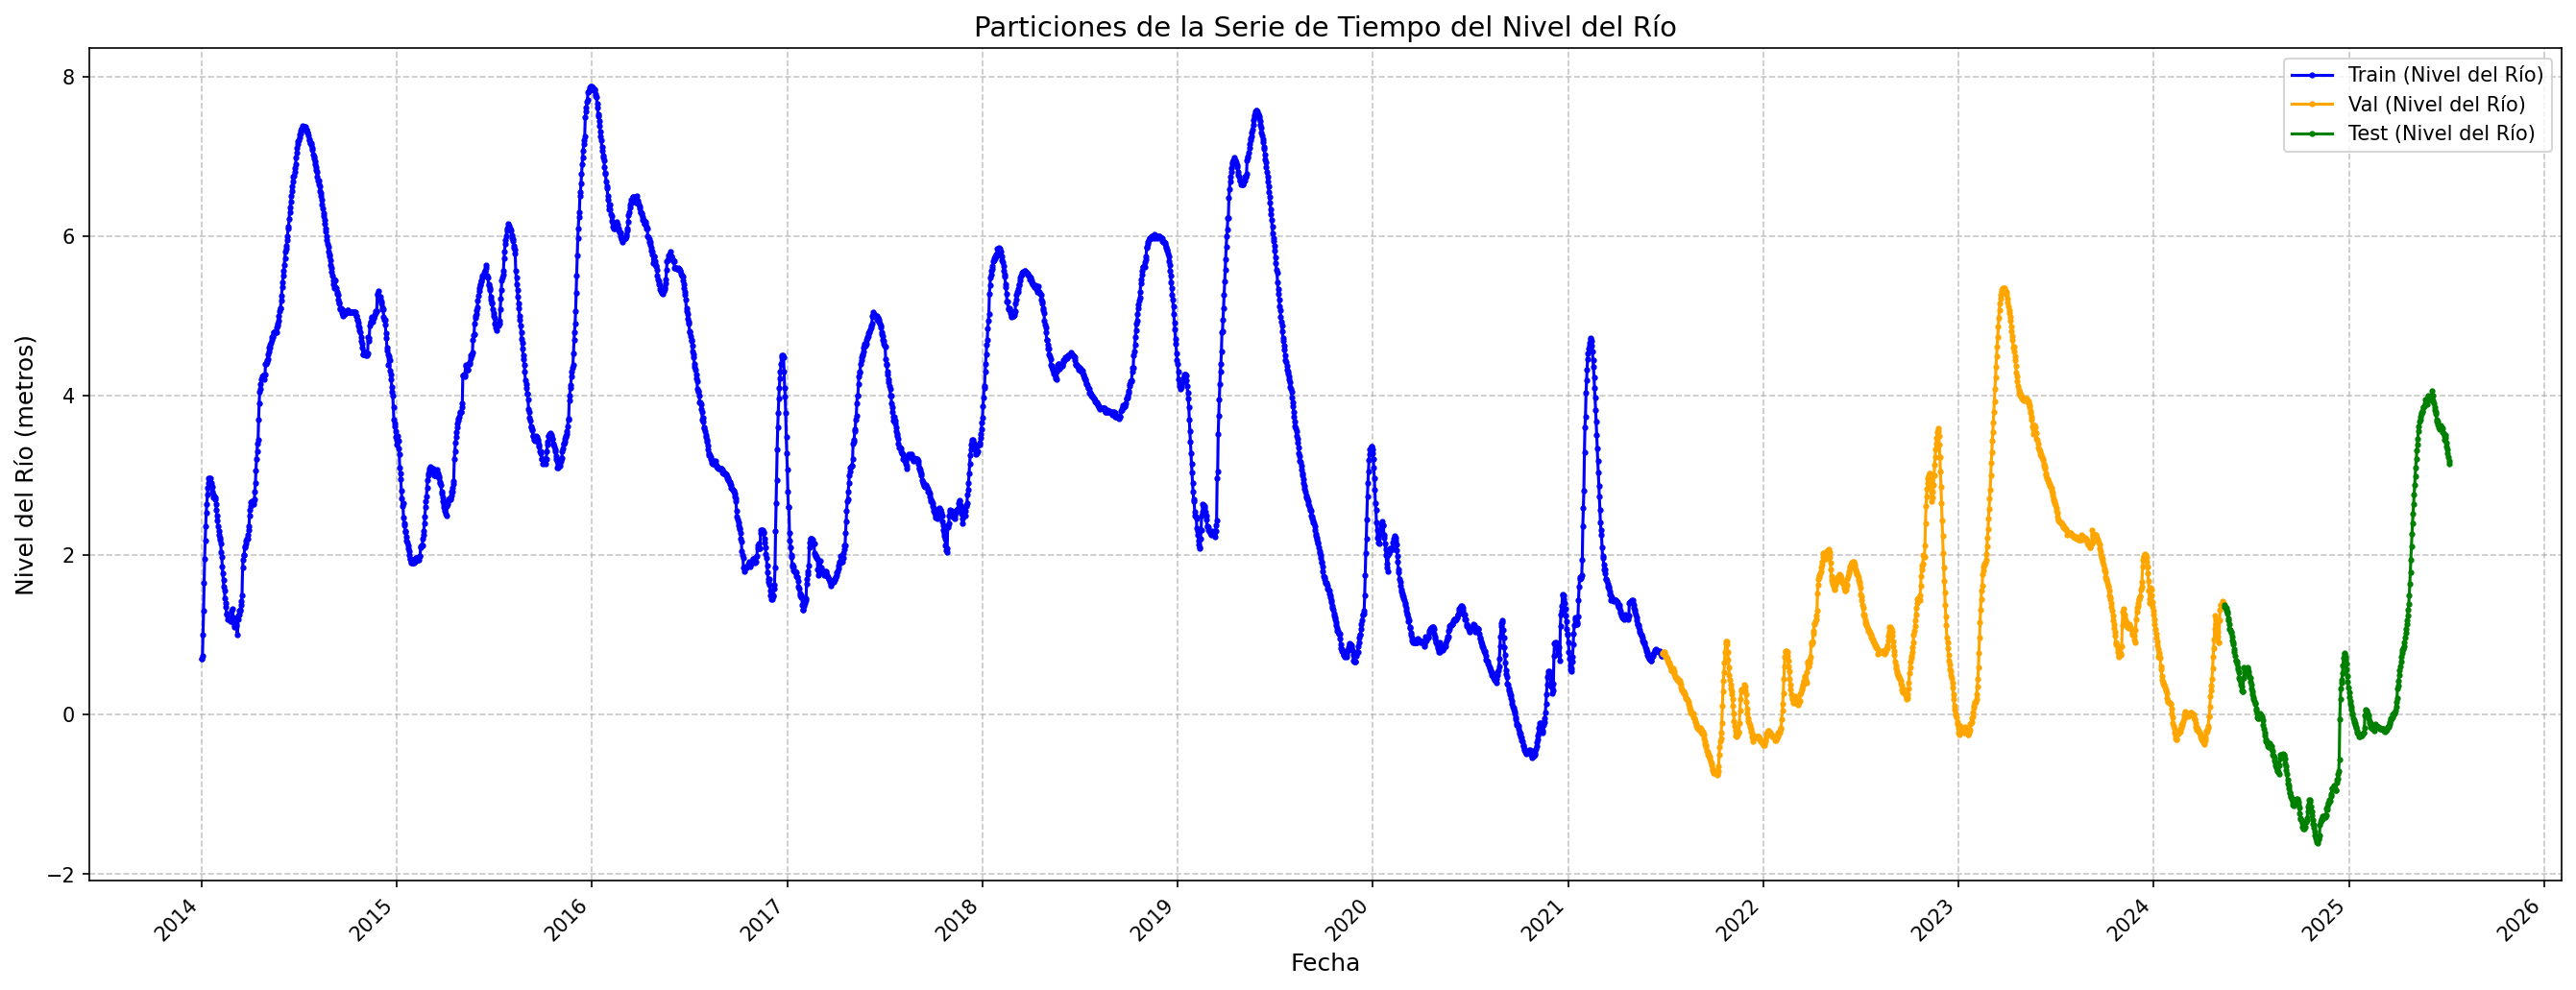
\includegraphics[width=0.82\textwidth]{../predicciones/prediccion_nivel_rio/resultados/grafico_01_particiones.png}
\end{frame}

% ============================================================
\begin{frame}{Predicci\'on del Nivel del R\'io a 730 D\'ias}
\centering
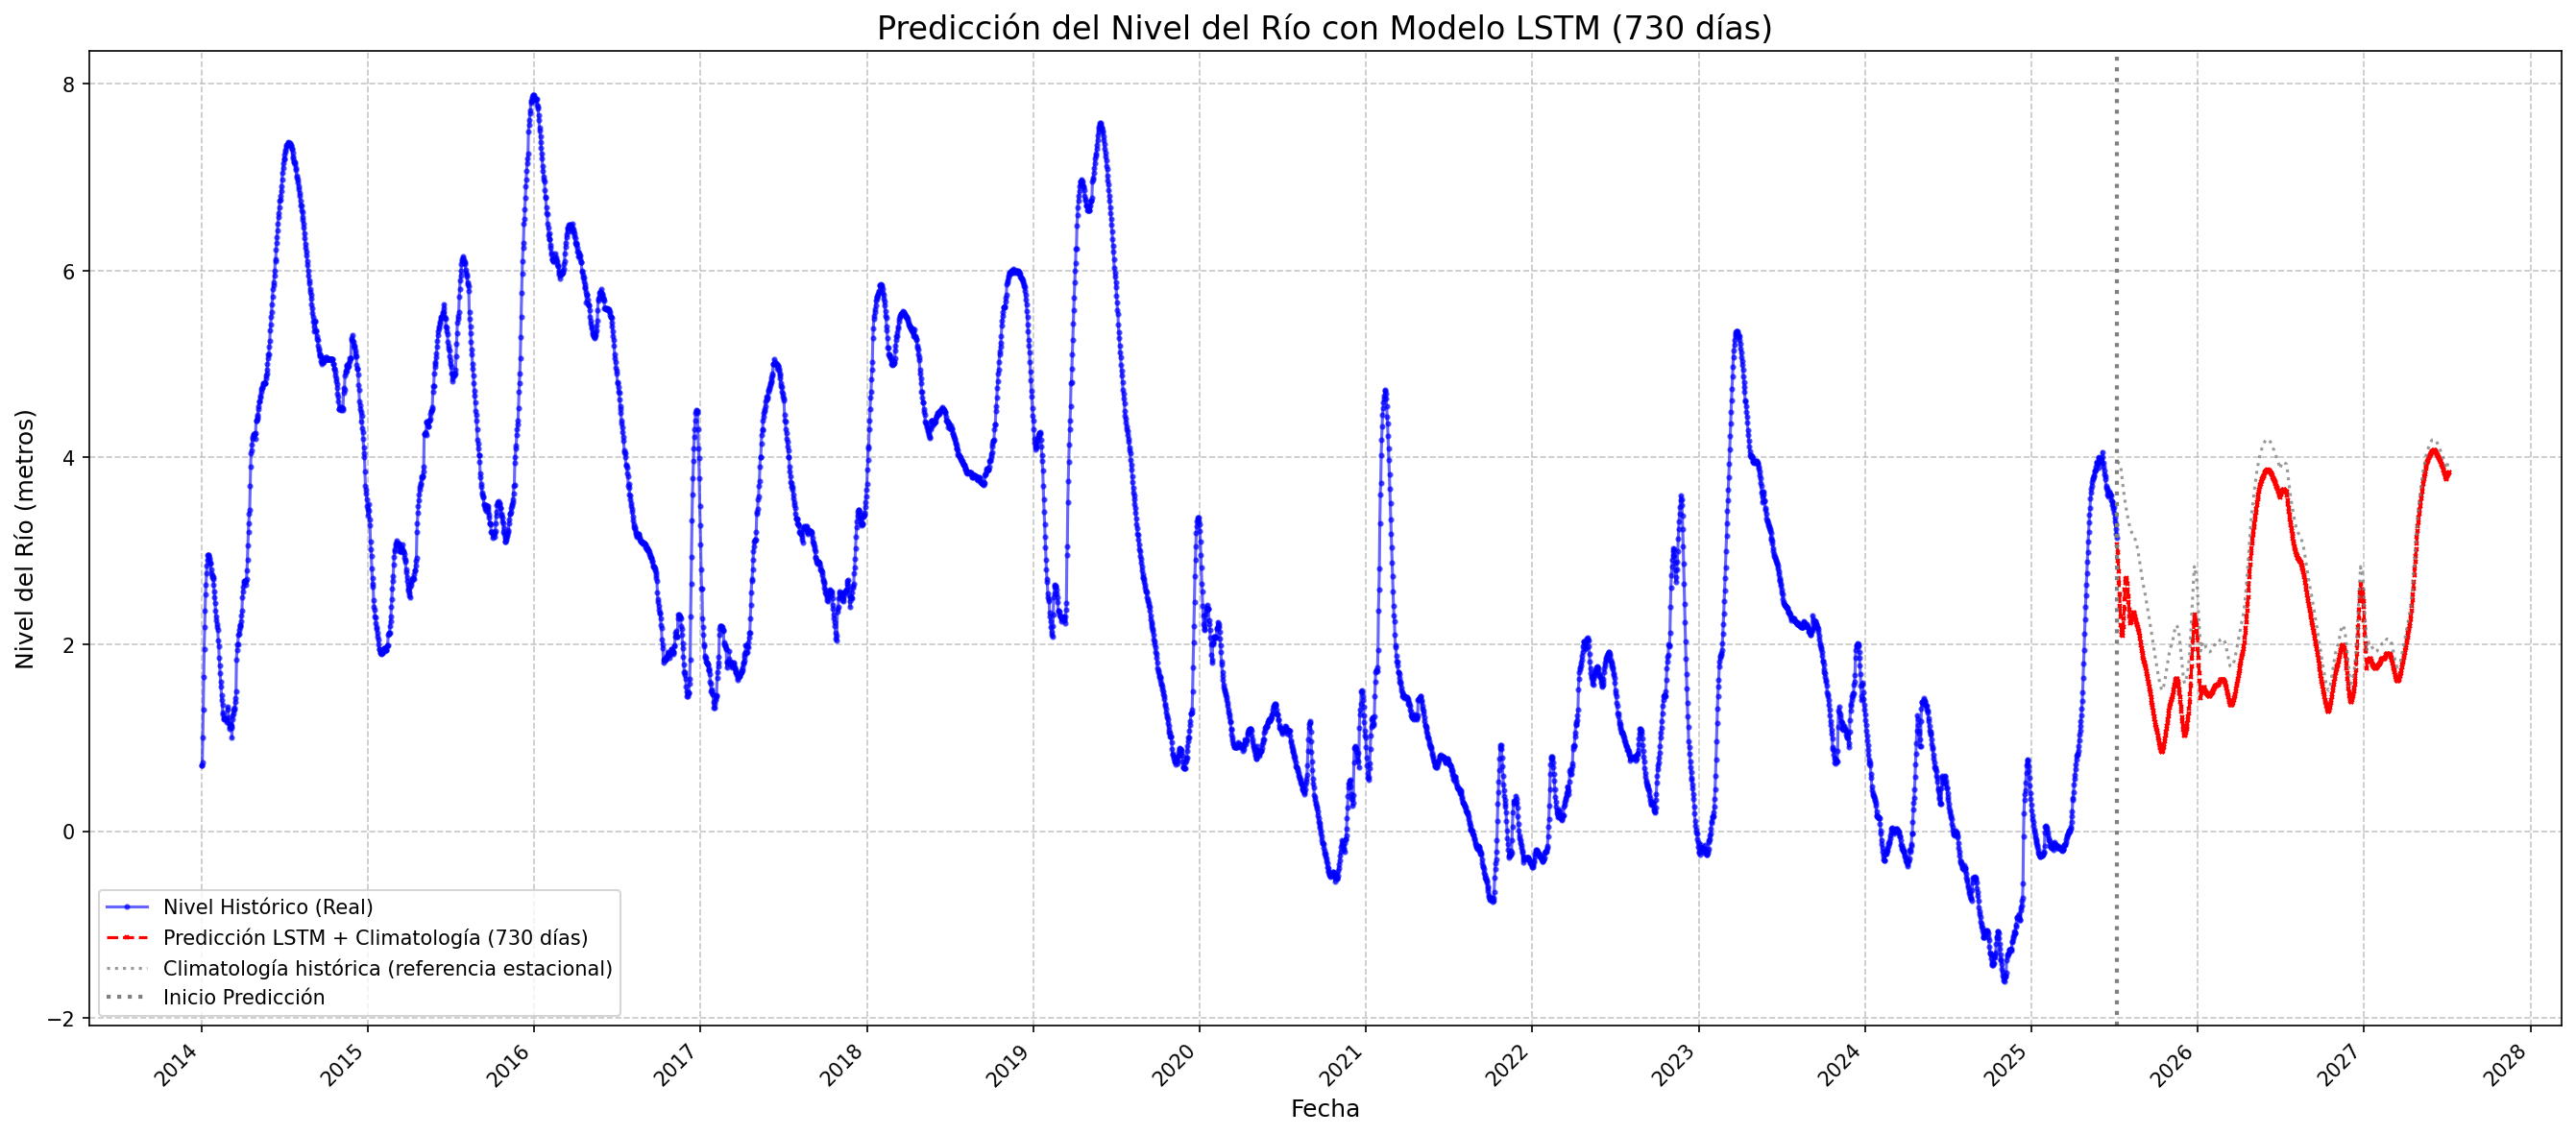
\includegraphics[width=0.82\textwidth]{../predicciones/prediccion_nivel_rio/resultados/grafico_08_historico_mas_prediccion.png}

\vspace{0.2cm}
\small Se extrae el \textbf{m\'inimo mensual} como variable ex\'ogena para los modelos de precios.
\end{frame}

% ============================================================
\section{Predicci\'on con SARIMAX}
% ============================================================

\begin{frame}{Modelo SARIMAX}
\begin{itemize}
  \item Modelo estad\'istico cl\'asico con variables ex\'ogenas.
  \item Selecci\'on autom\'atica de \'ordenes: \texttt{auto\_arima} (minimizar AIC).
  \item Variables ex\'ogenas: nivel del r\'io + cuarentena COVID-19.
  \item Validaci\'on por \textbf{ventana deslizante} (rolling forecast).
\end{itemize}

\vspace{0.3cm}
\begin{alertblock}{Resultado de auto\_arima (ambos materiales)}
\centering
\Large $\text{ARIMA}(0,1,0)(0,0,0)_{12}$\\[0.2cm]
\normalsize Equivale a un \textbf{paseo aleatorio}: el pron\'ostico es el valor del mes anterior.\\
Variables ex\'ogenas \textbf{no significativas}: nivel r\'io ($p=0{,}894$), cuarentena ($p=1{,}000$).
\end{alertblock}
\end{frame}

% ============================================================
\begin{frame}{SARIMAX --- Cemento}
\centering
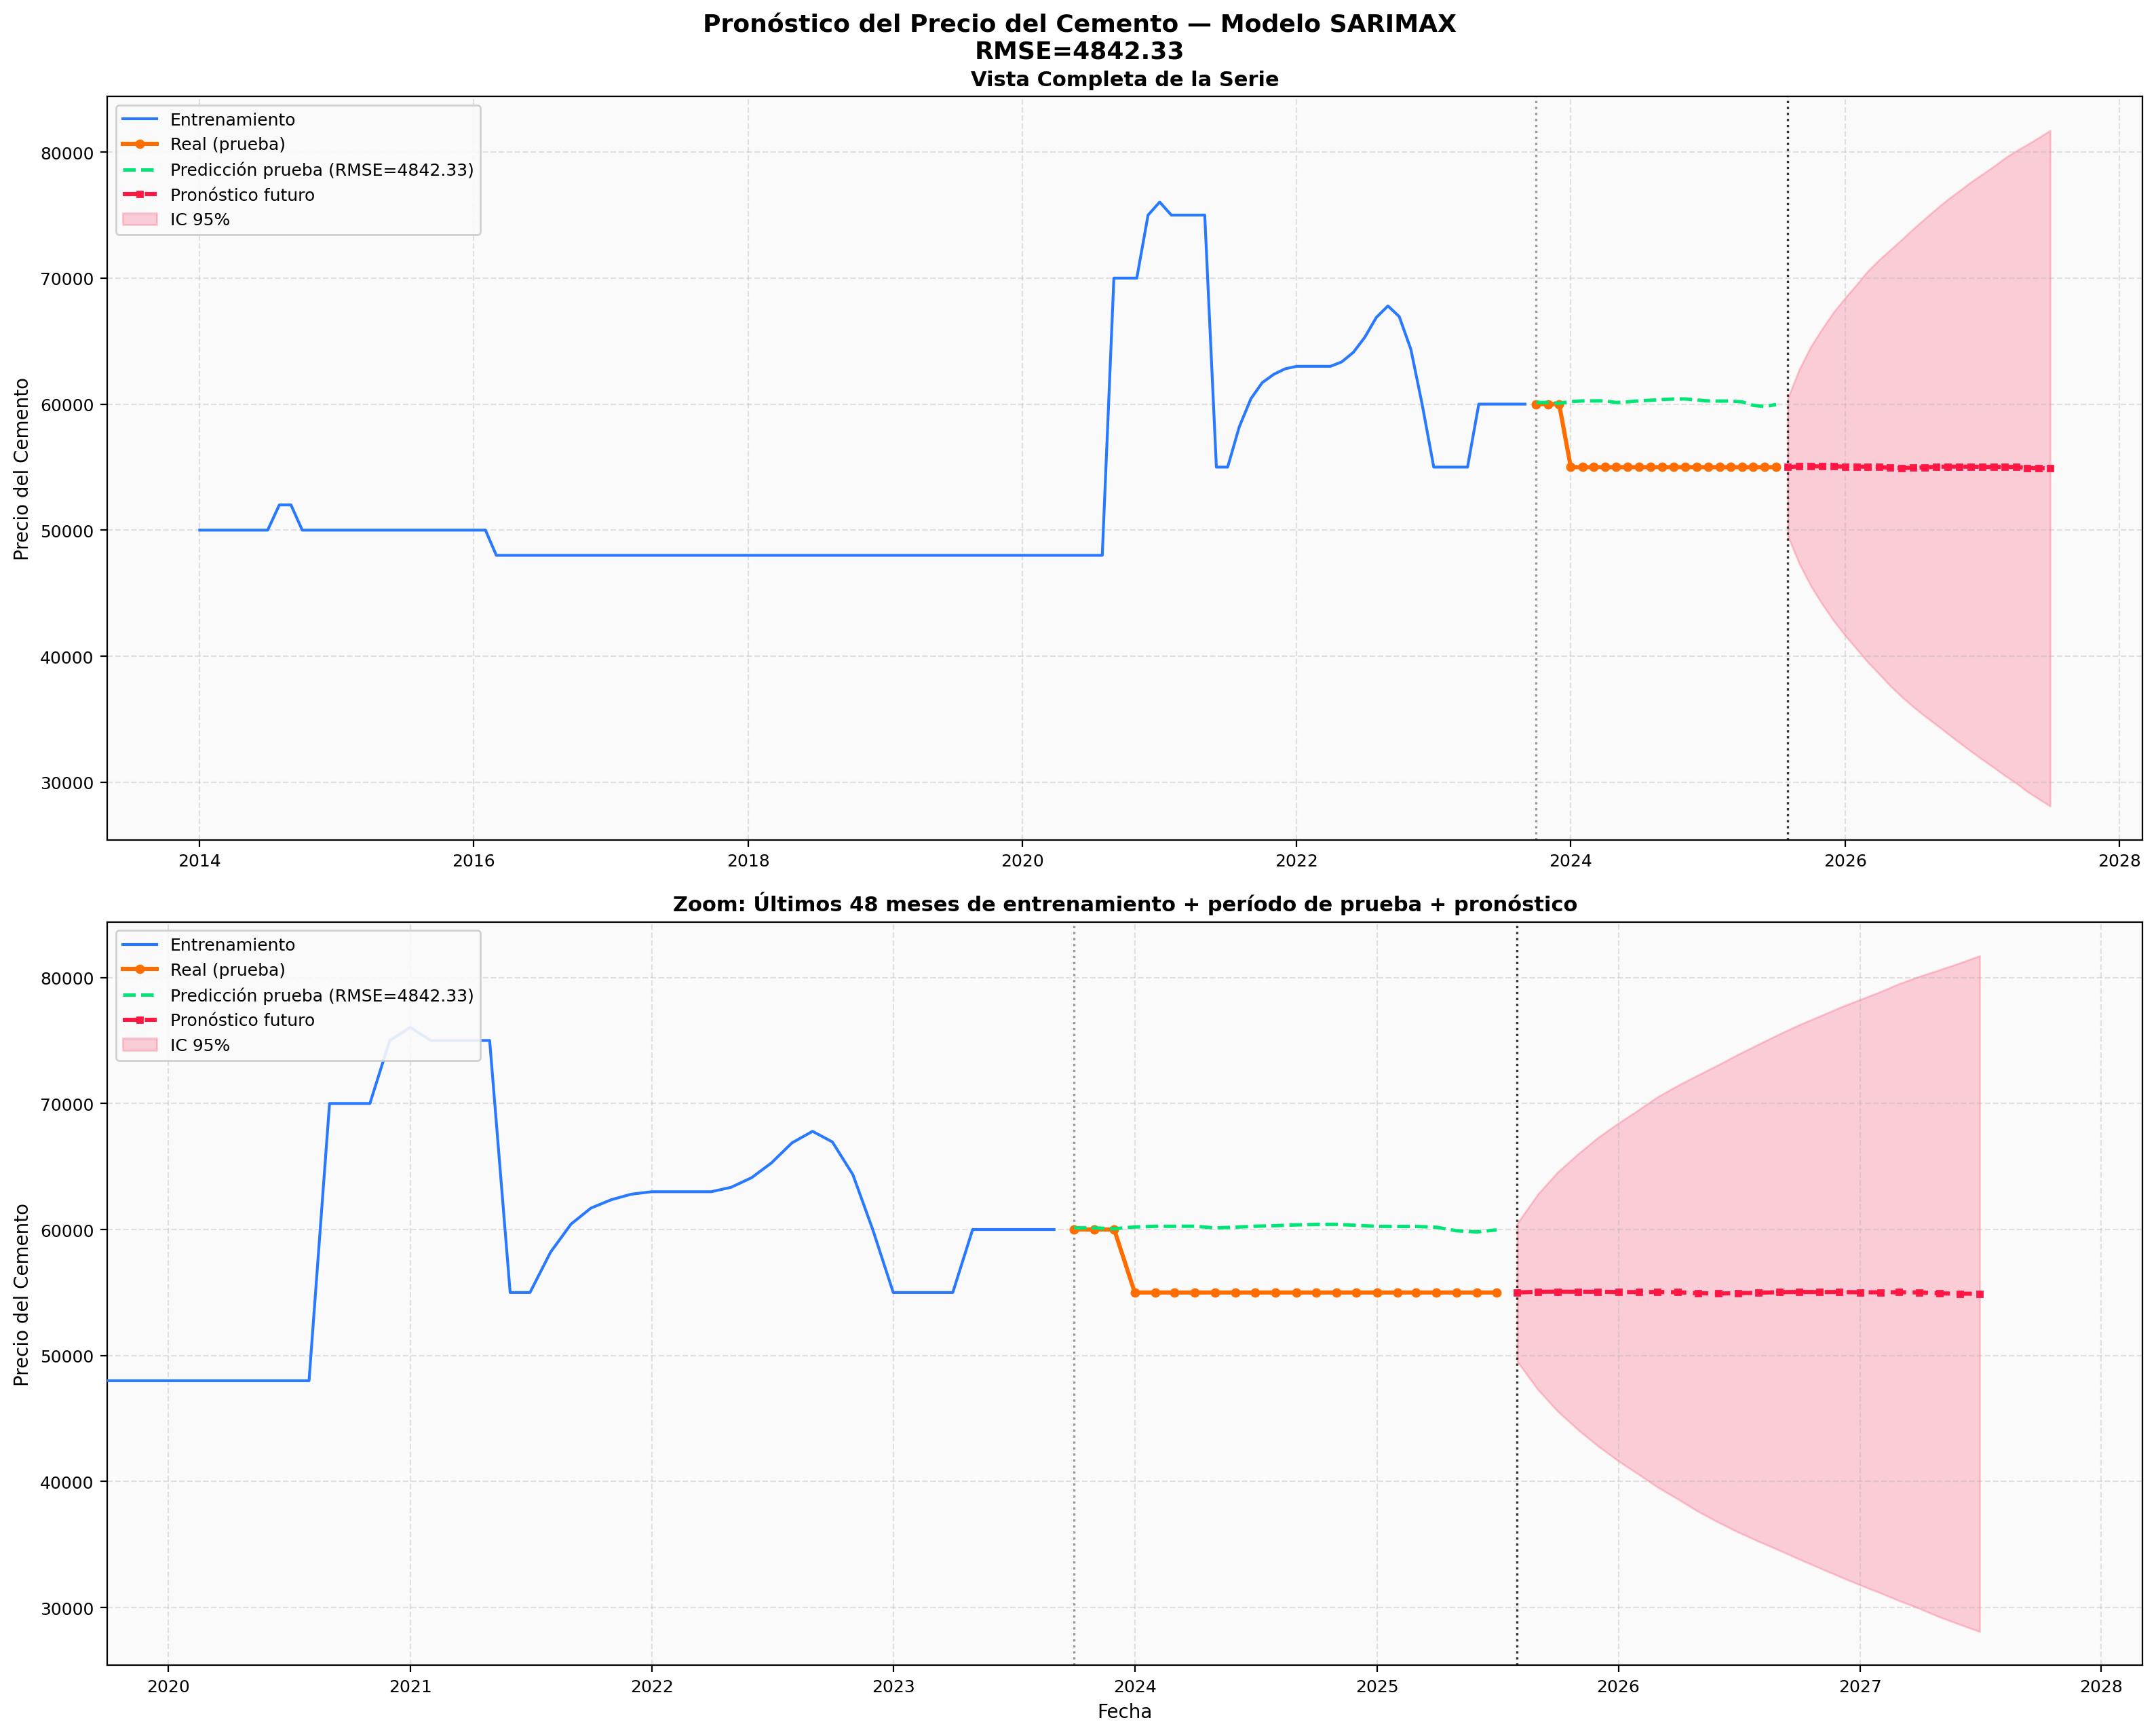
\includegraphics[width=0.78\textwidth]{../predicciones/prediccion_sarimax_cemento/resultados_sarimax_cemento/graficos/06_pronostico_completo.png}

\vspace{0.1cm}
\begin{columns}
\begin{column}{0.5\textwidth}
\begin{itemize}\small
  \item RMSE Validaci\'on: 4.170,12 Gs.
  \item RMSE Prueba: 4.840,06 Gs.
\end{itemize}
\end{column}
\begin{column}{0.5\textwidth}
\begin{itemize}\small
  \item Par\'ametros: 3
  \item Pron\'ostico: $\sim$55.000 Gs.
\end{itemize}
\end{column}
\end{columns}
\end{frame}

% ============================================================
\begin{frame}{SARIMAX --- Ladrillo}
\centering
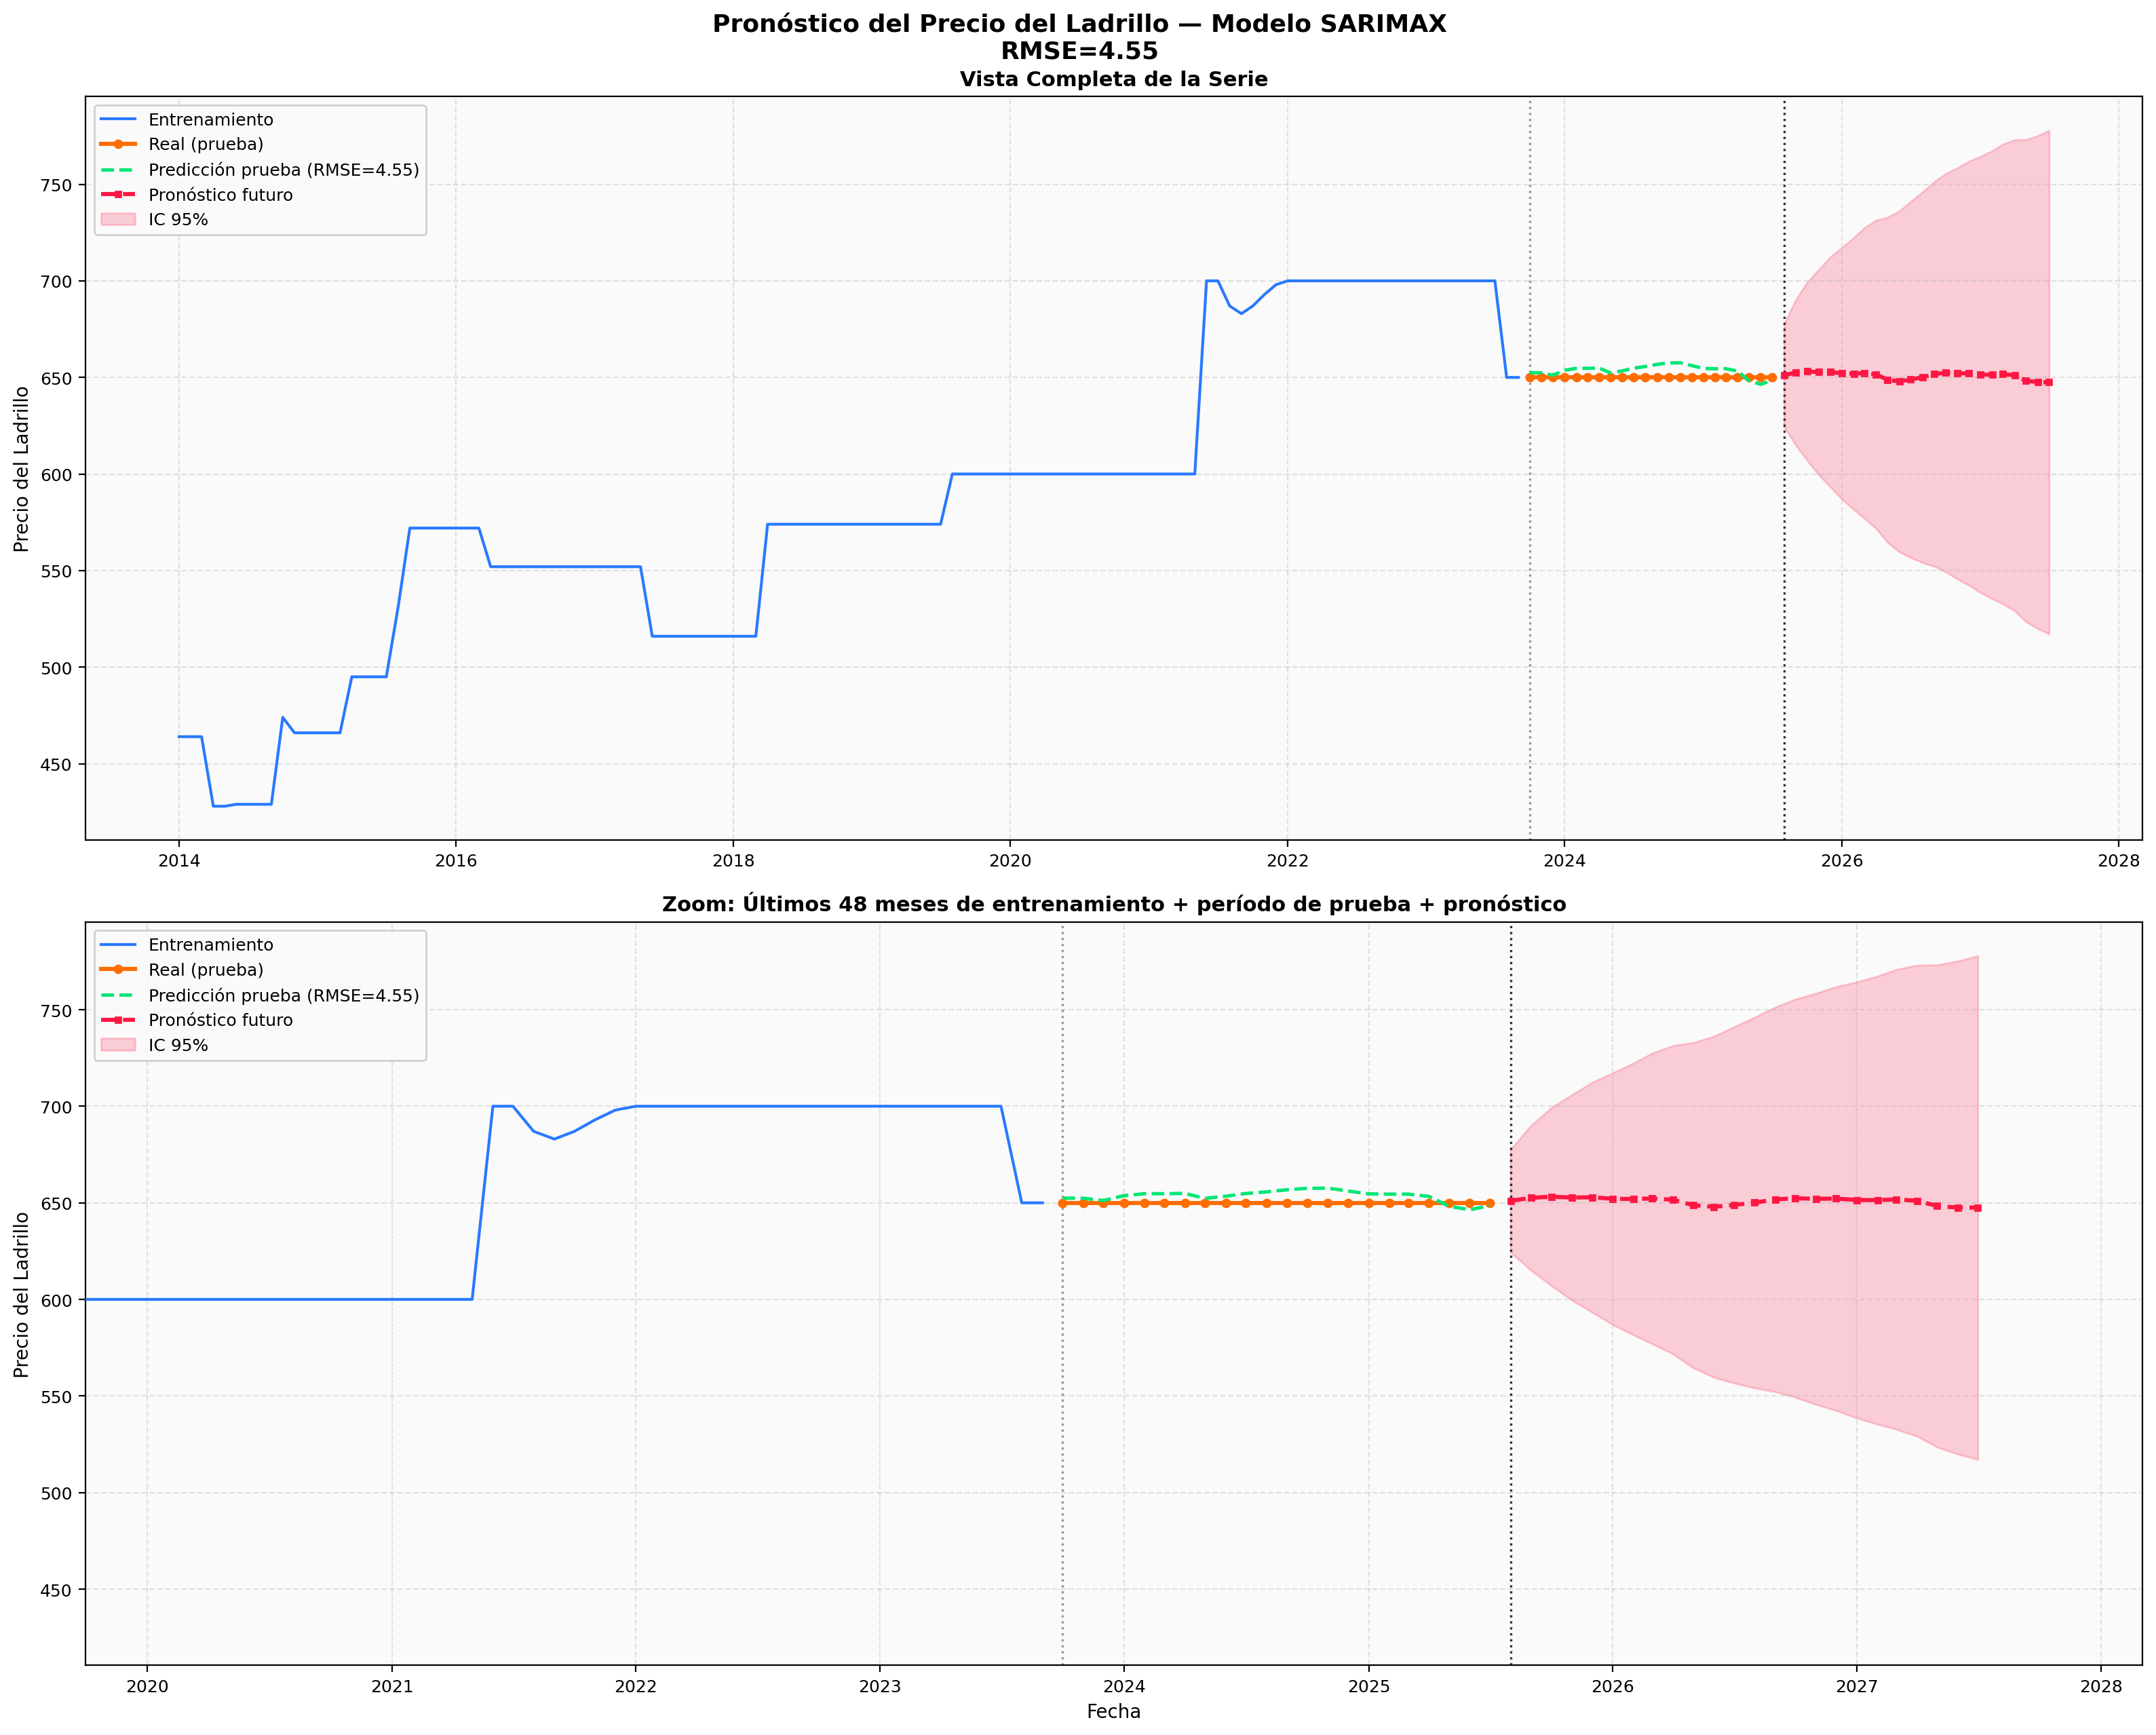
\includegraphics[width=0.78\textwidth]{../predicciones/prediccion_sarimax_ladrillo/resultados_sarimax_ladrillo/graficos/06_pronostico_completo.png}

\vspace{0.1cm}
\begin{columns}
\begin{column}{0.5\textwidth}
\begin{itemize}\small
  \item RMSE Validaci\'on: 14,92 Gs.
  \item RMSE Prueba: 4,55 Gs.
\end{itemize}
\end{column}
\begin{column}{0.5\textwidth}
\begin{itemize}\small
  \item Par\'ametros: 3
  \item Pron\'ostico: $\sim$651 Gs.
\end{itemize}
\end{column}
\end{columns}
\end{frame}

% ============================================================
\section{Predicci\'on con LSTM}
% ============================================================

\begin{frame}{Partici\'on del Conjunto de Datos --- Materiales}
\centering
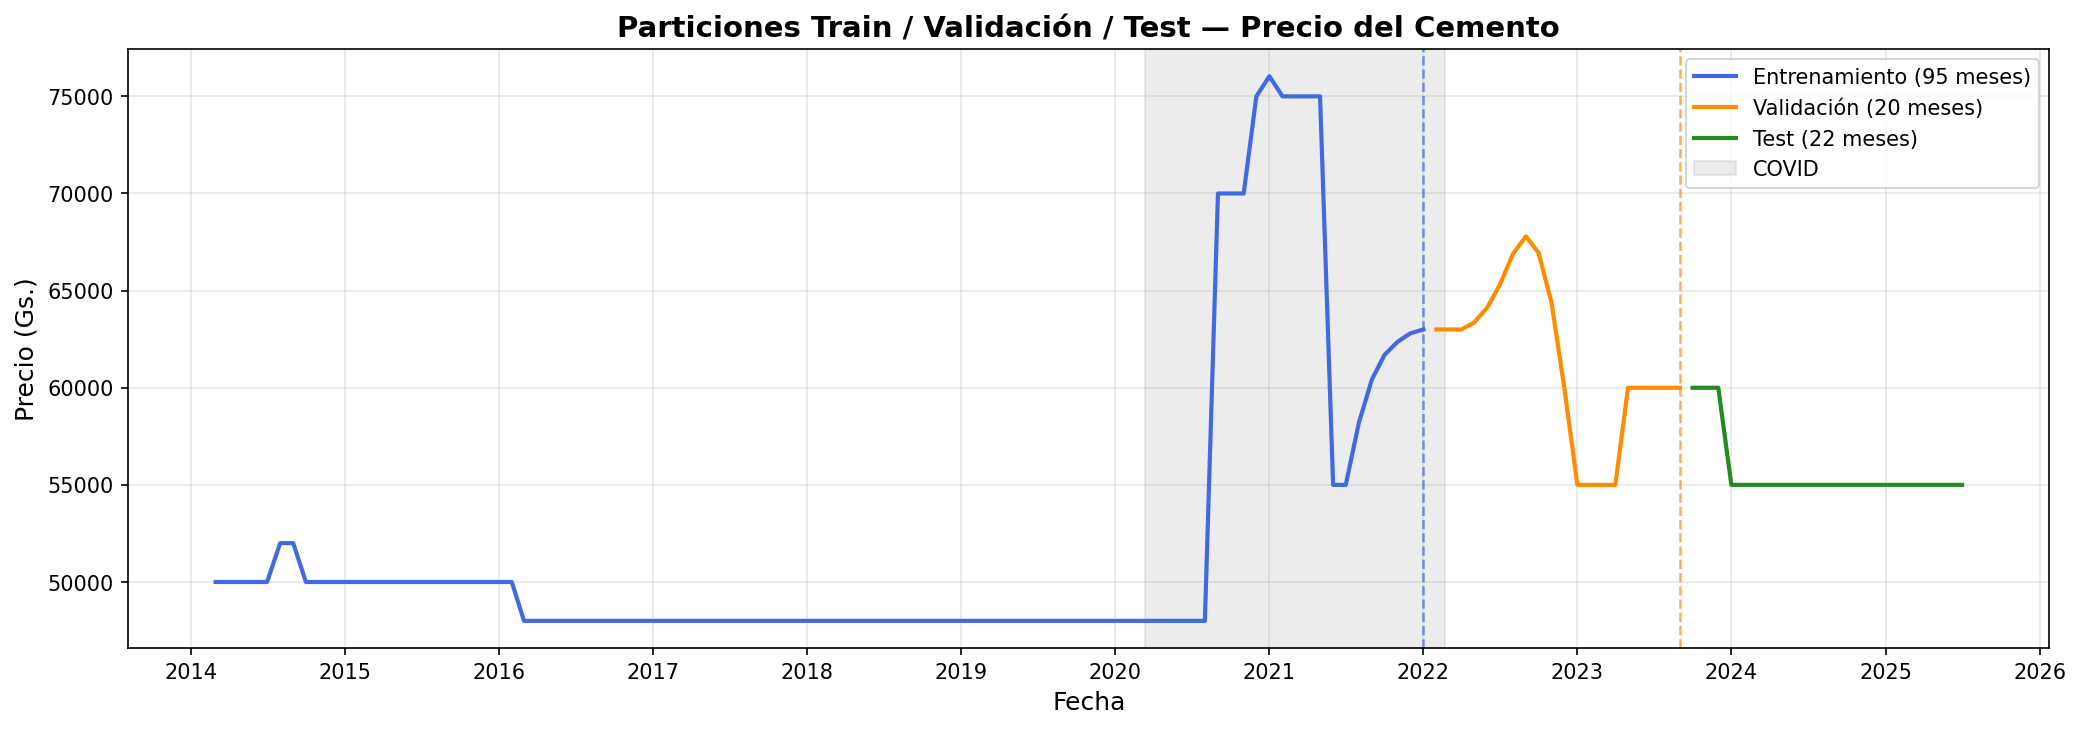
\includegraphics[width=0.78\textwidth]{../predicciones/prediccion_cemento_lstm/resultados_con_covid/entrenamiento_01_particiones.png}

\vspace{0.2cm}
\small Partici\'on cronol\'ogica: 97 meses (train) + 20 meses (val) + 22 meses (test).\\
Zona sombreada: per\'iodo de cuarentena por COVID-19.
\end{frame}

% ============================================================
\begin{frame}{LSTM Cemento --- Sin Confinamiento}
\centering
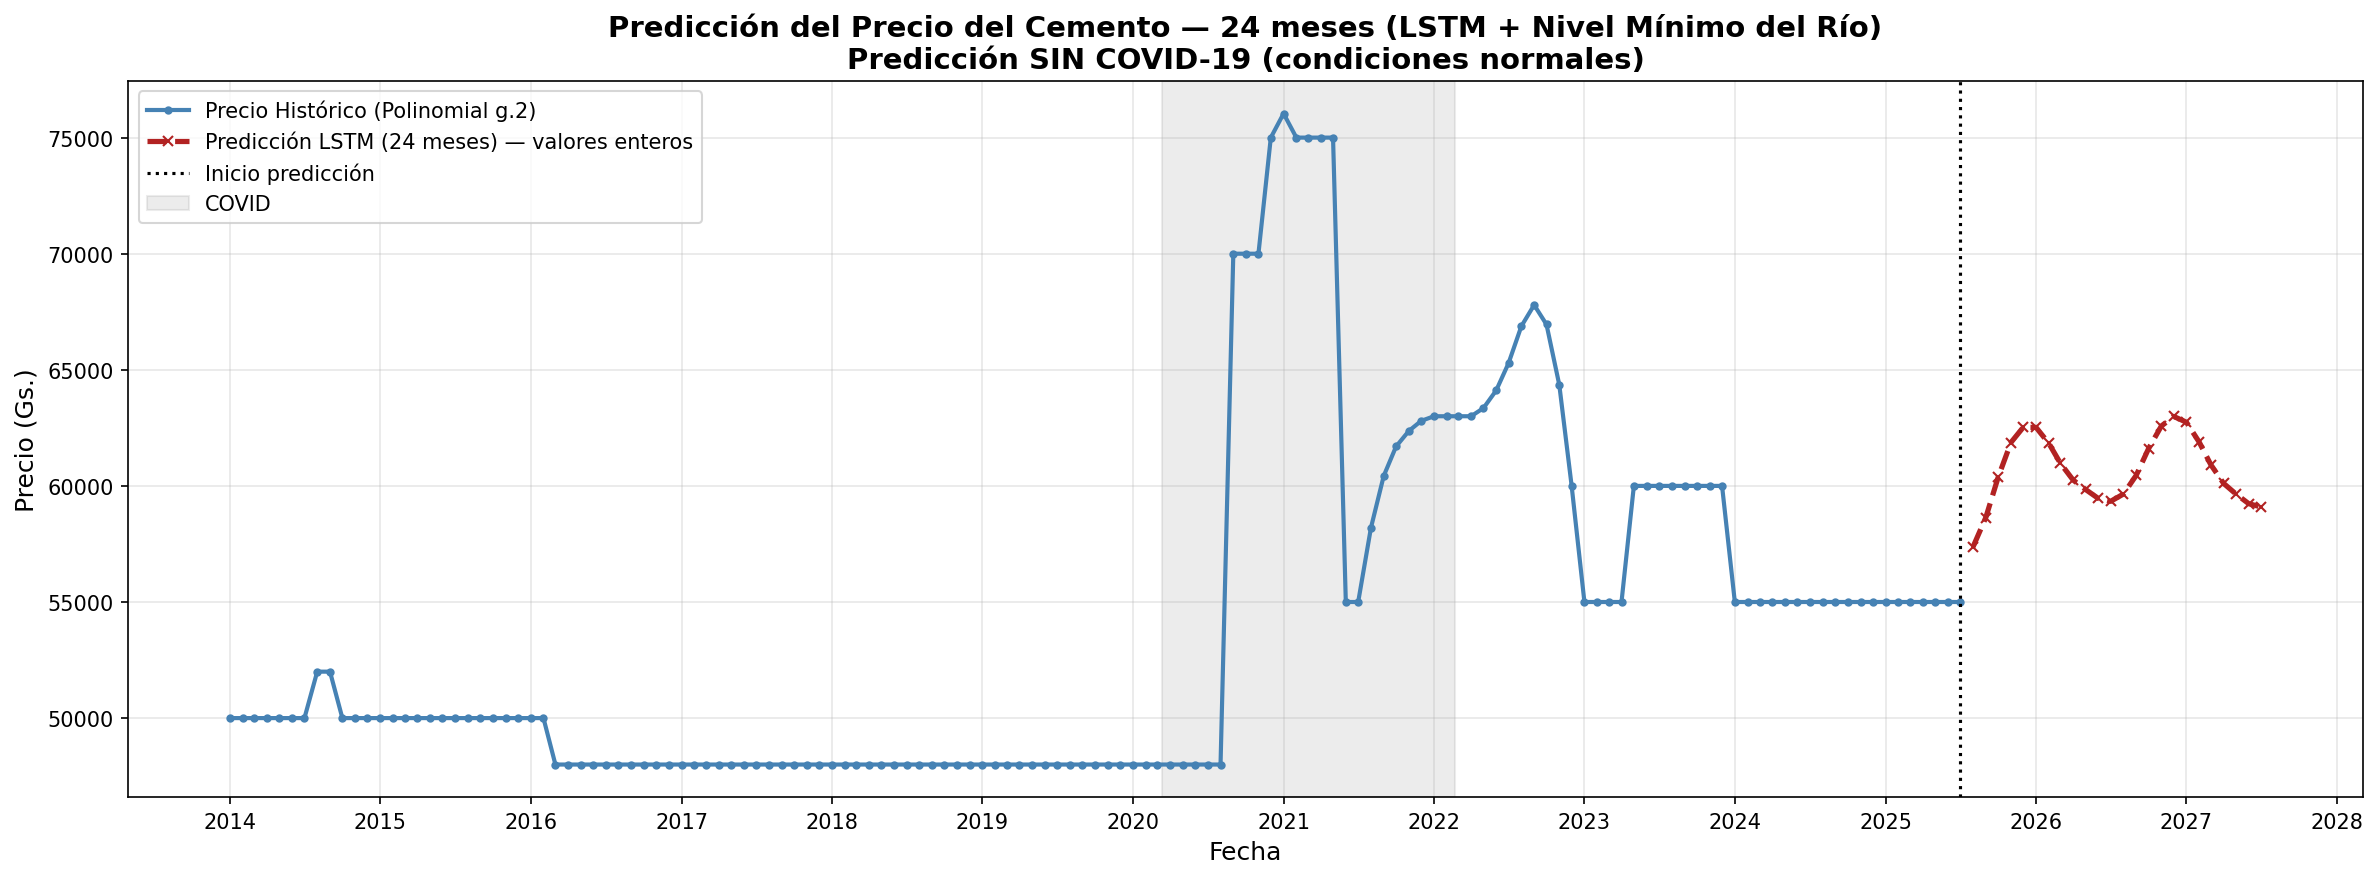
\includegraphics[width=0.75\textwidth]{../predicciones/prediccion_cemento_lstm/resultados_sin_covid/final_06_prediccion_futura_completa.png}

\vspace{0.1cm}
\begin{columns}
\begin{column}{0.5\textwidth}
\begin{itemize}\small
  \item RMSE Test: 4.394,96 Gs.
  \item Par\'ametros: 36.481
  \item Arquitectura bidireccional
\end{itemize}
\end{column}
\begin{column}{0.5\textwidth}
\begin{itemize}\small
  \item Adam (lr=0,0086)
  \item Lookback: 3 meses
  \item Pron\'ostico: 57.372--62.992 Gs.
\end{itemize}
\end{column}
\end{columns}
\end{frame}

% ============================================================
\begin{frame}{LSTM Cemento --- Con Confinamiento}
\centering
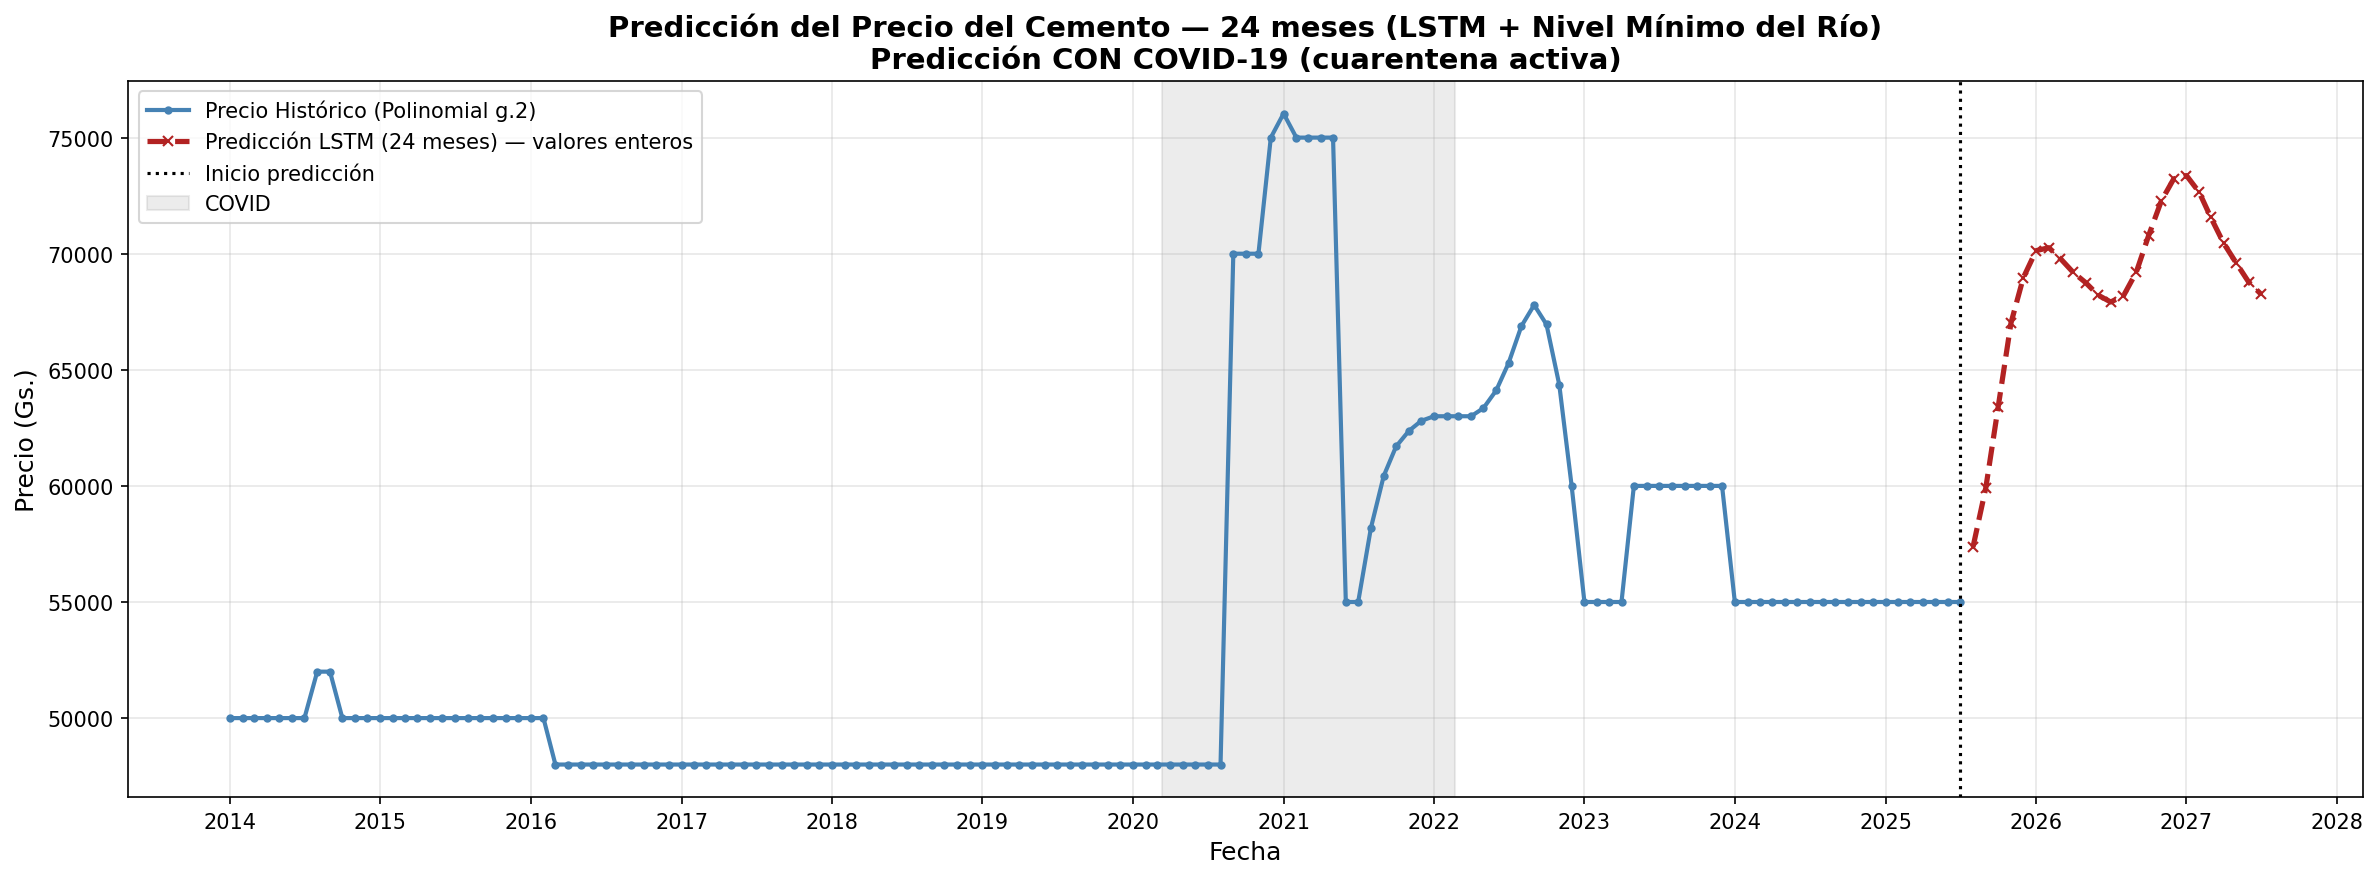
\includegraphics[width=0.75\textwidth]{../predicciones/prediccion_cemento_lstm/resultados_con_covid/final_06_prediccion_futura_completa.png}

\vspace{0.1cm}
\begin{columns}
\begin{column}{0.5\textwidth}
\begin{itemize}\small
  \item RMSE Test: 4.394,96 Gs.
  \item Misma arquitectura bidireccional
  \item 36.481 par\'ametros
\end{itemize}
\end{column}
\begin{column}{0.5\textwidth}
\begin{itemize}\small
  \item Pron\'ostico: 57.372--73.366 Gs.
  \item \textbf{+16,5\,\%} en l\'imite superior
  \item Consistente con 2020--2022
\end{itemize}
\end{column}
\end{columns}
\end{frame}

% ============================================================
\begin{frame}{LSTM Ladrillo --- Sin Confinamiento}
\centering
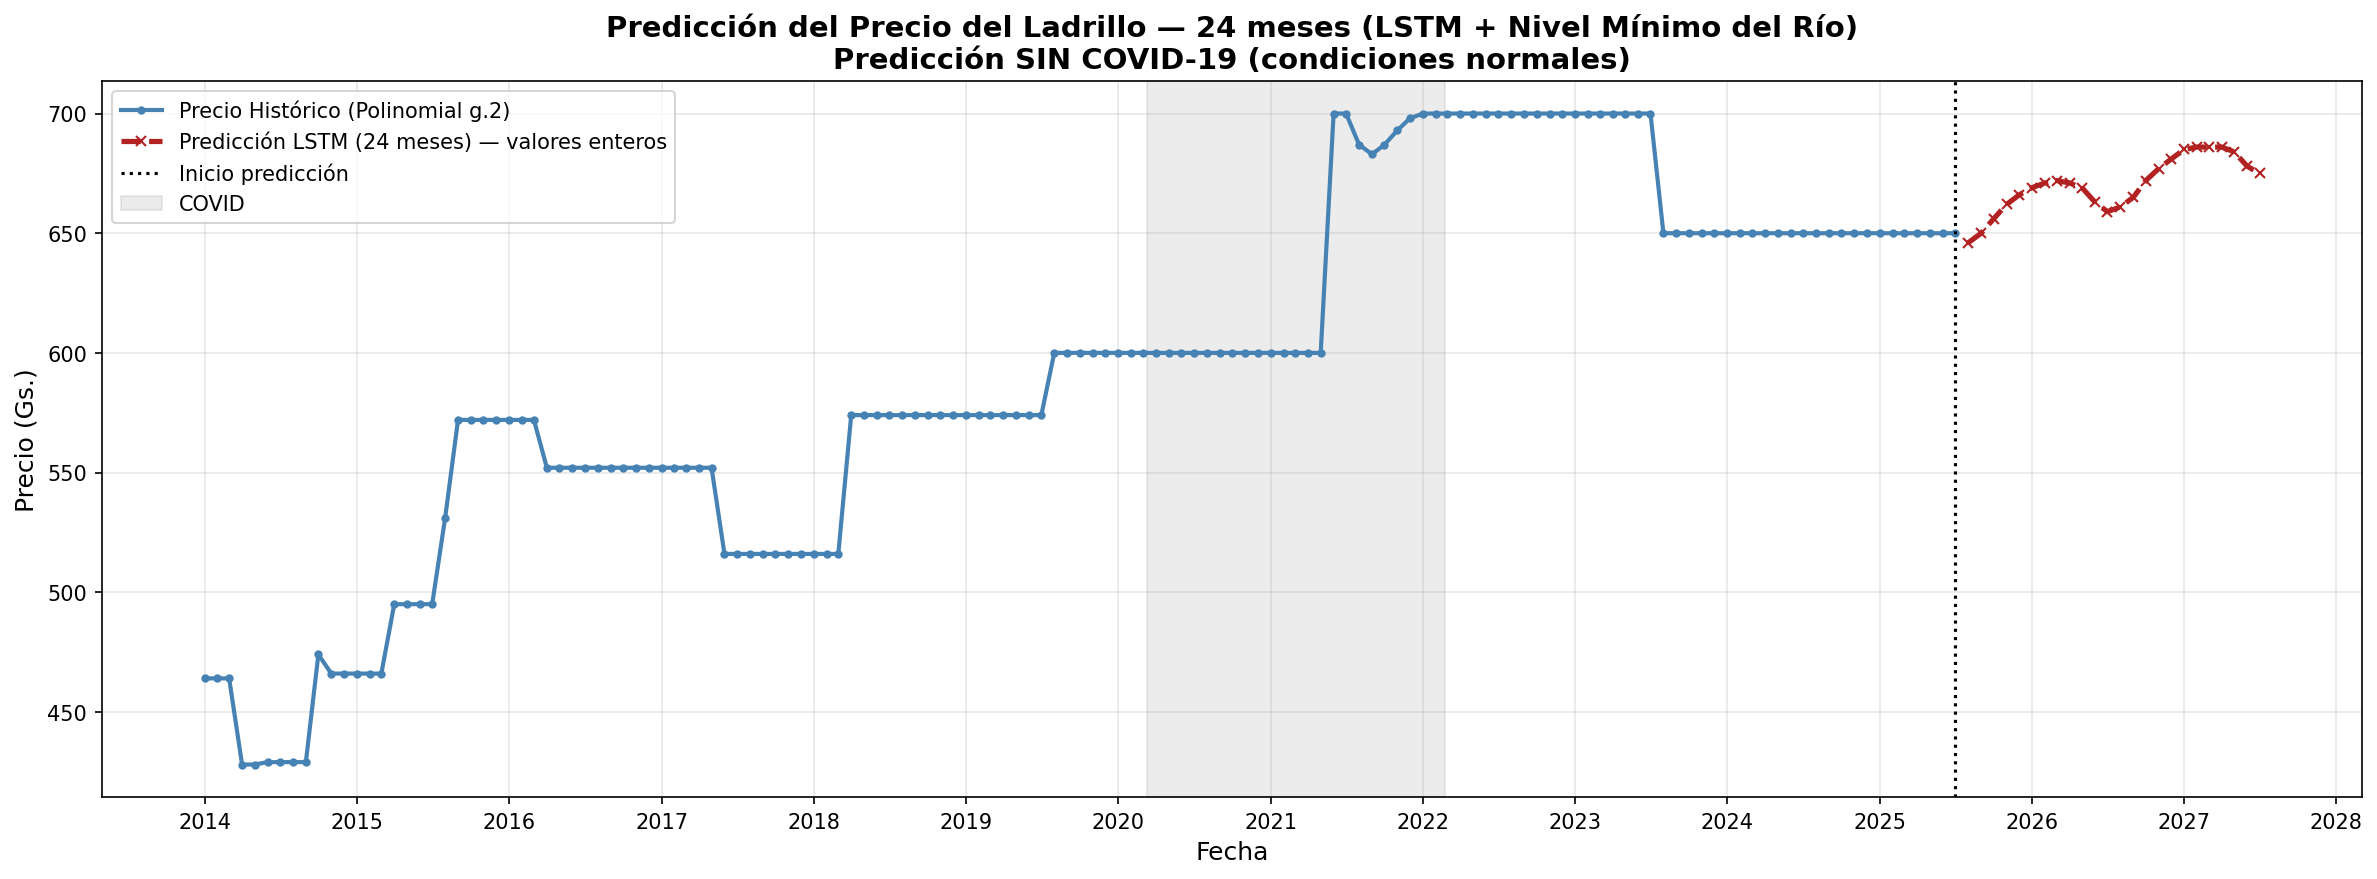
\includegraphics[width=0.75\textwidth]{../predicciones/prediccion_ladrillo_lstm/resultados_sin_covid/final_06_prediccion_futura_completa.png}

\vspace{0.1cm}
\begin{columns}
\begin{column}{0.5\textwidth}
\begin{itemize}\small
  \item RMSE Test: 7,68 Gs.
  \item Par\'ametros: 18.241
  \item Unidireccional
\end{itemize}
\end{column}
\begin{column}{0.5\textwidth}
\begin{itemize}\small
  \item AdamW (lr=0,0086)
  \item Lookback: 6 meses
  \item Pron\'ostico: 646--686 Gs.
\end{itemize}
\end{column}
\end{columns}
\end{frame}

% ============================================================
\begin{frame}{LSTM Ladrillo --- Con Confinamiento}
\centering
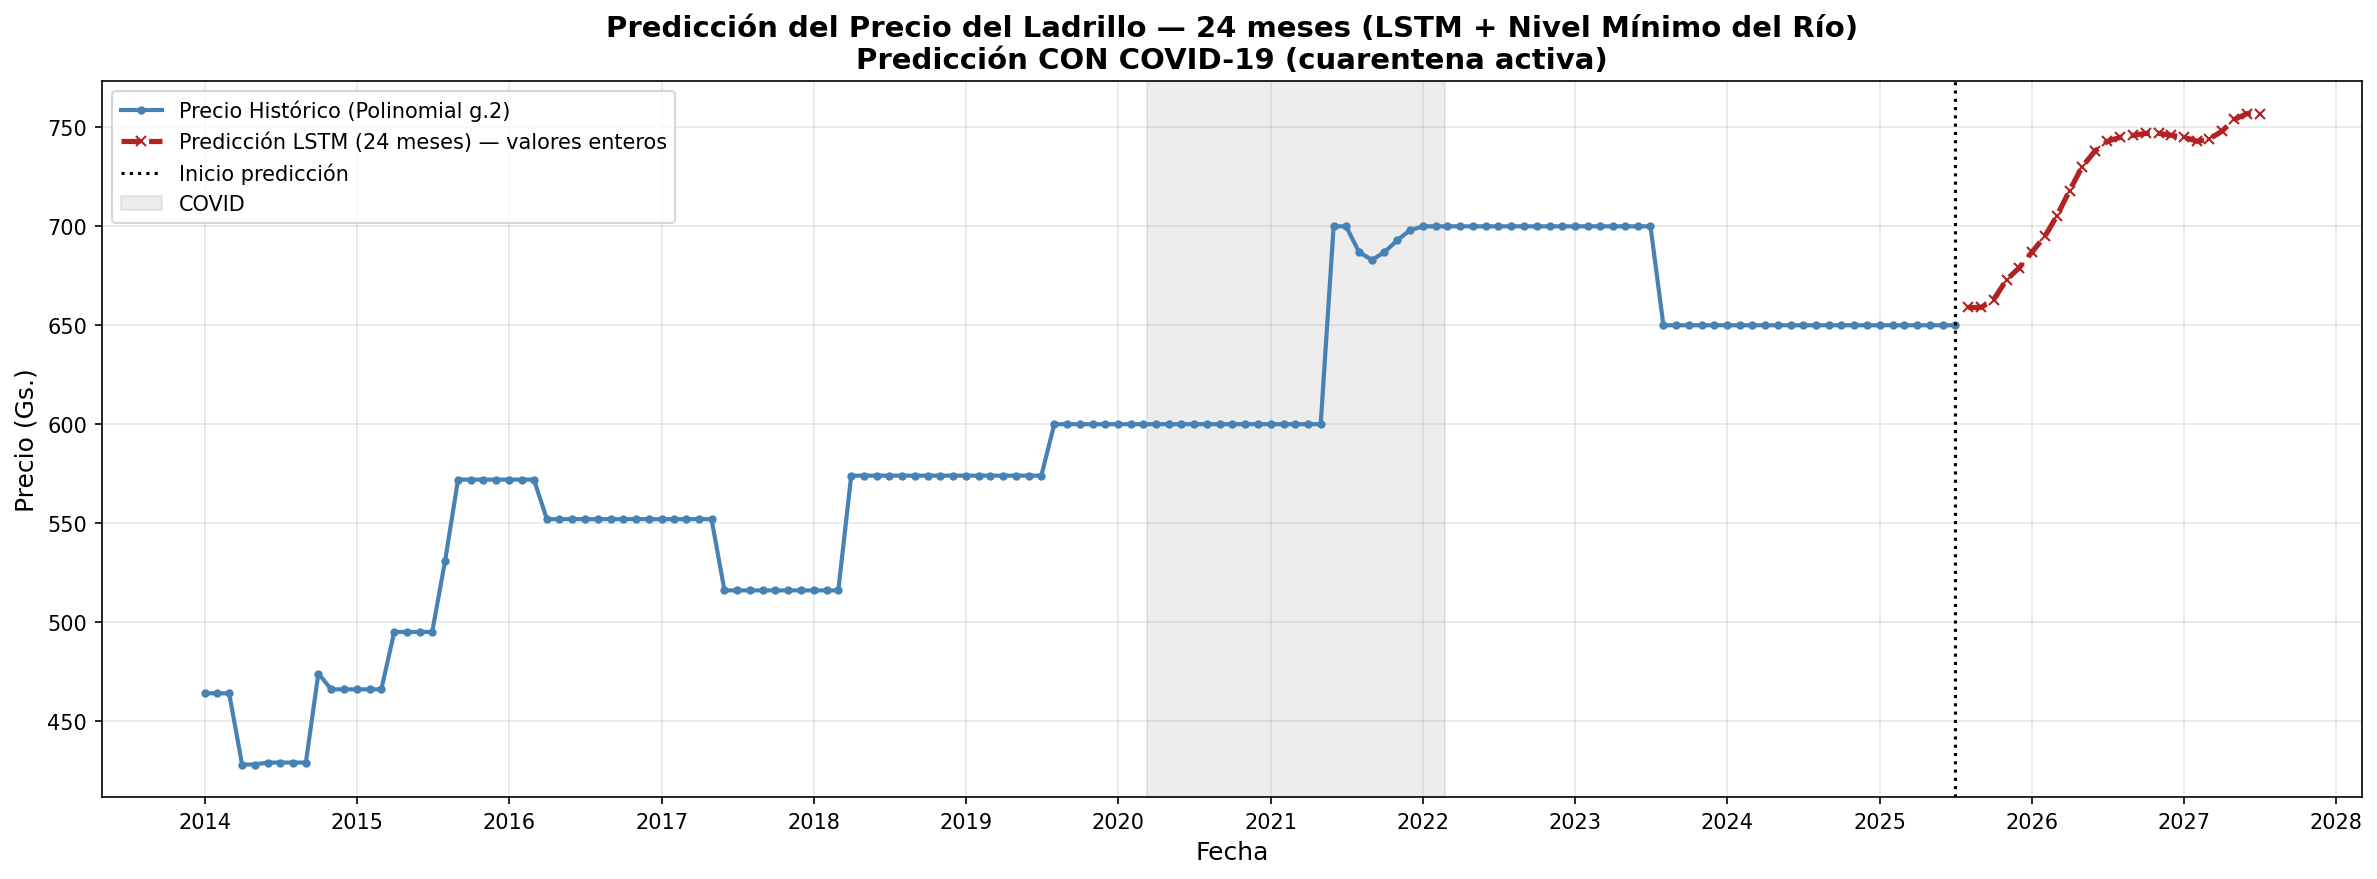
\includegraphics[width=0.75\textwidth]{../predicciones/prediccion_ladrillo_lstm/resultados_con_covid/final_06_prediccion_futura_completa.png}

\vspace{0.1cm}
\begin{columns}
\begin{column}{0.5\textwidth}
\begin{itemize}\small
  \item RMSE Test: 6,62 Gs.
  \item Par\'ametros: 36.481
  \item Bidireccional (distinta arq.)
\end{itemize}
\end{column}
\begin{column}{0.5\textwidth}
\begin{itemize}\small
  \item RMSprop (lr=0,0027)
  \item Pron\'ostico: 656--758 Gs.
  \item \textbf{+10,5\,\%} en l\'imite superior
\end{itemize}
\end{column}
\end{columns}
\end{frame}

% ============================================================
\section{Predicci\'on con GRU}
% ============================================================

\begin{frame}{GRU Cemento --- Sin Confinamiento}
\centering
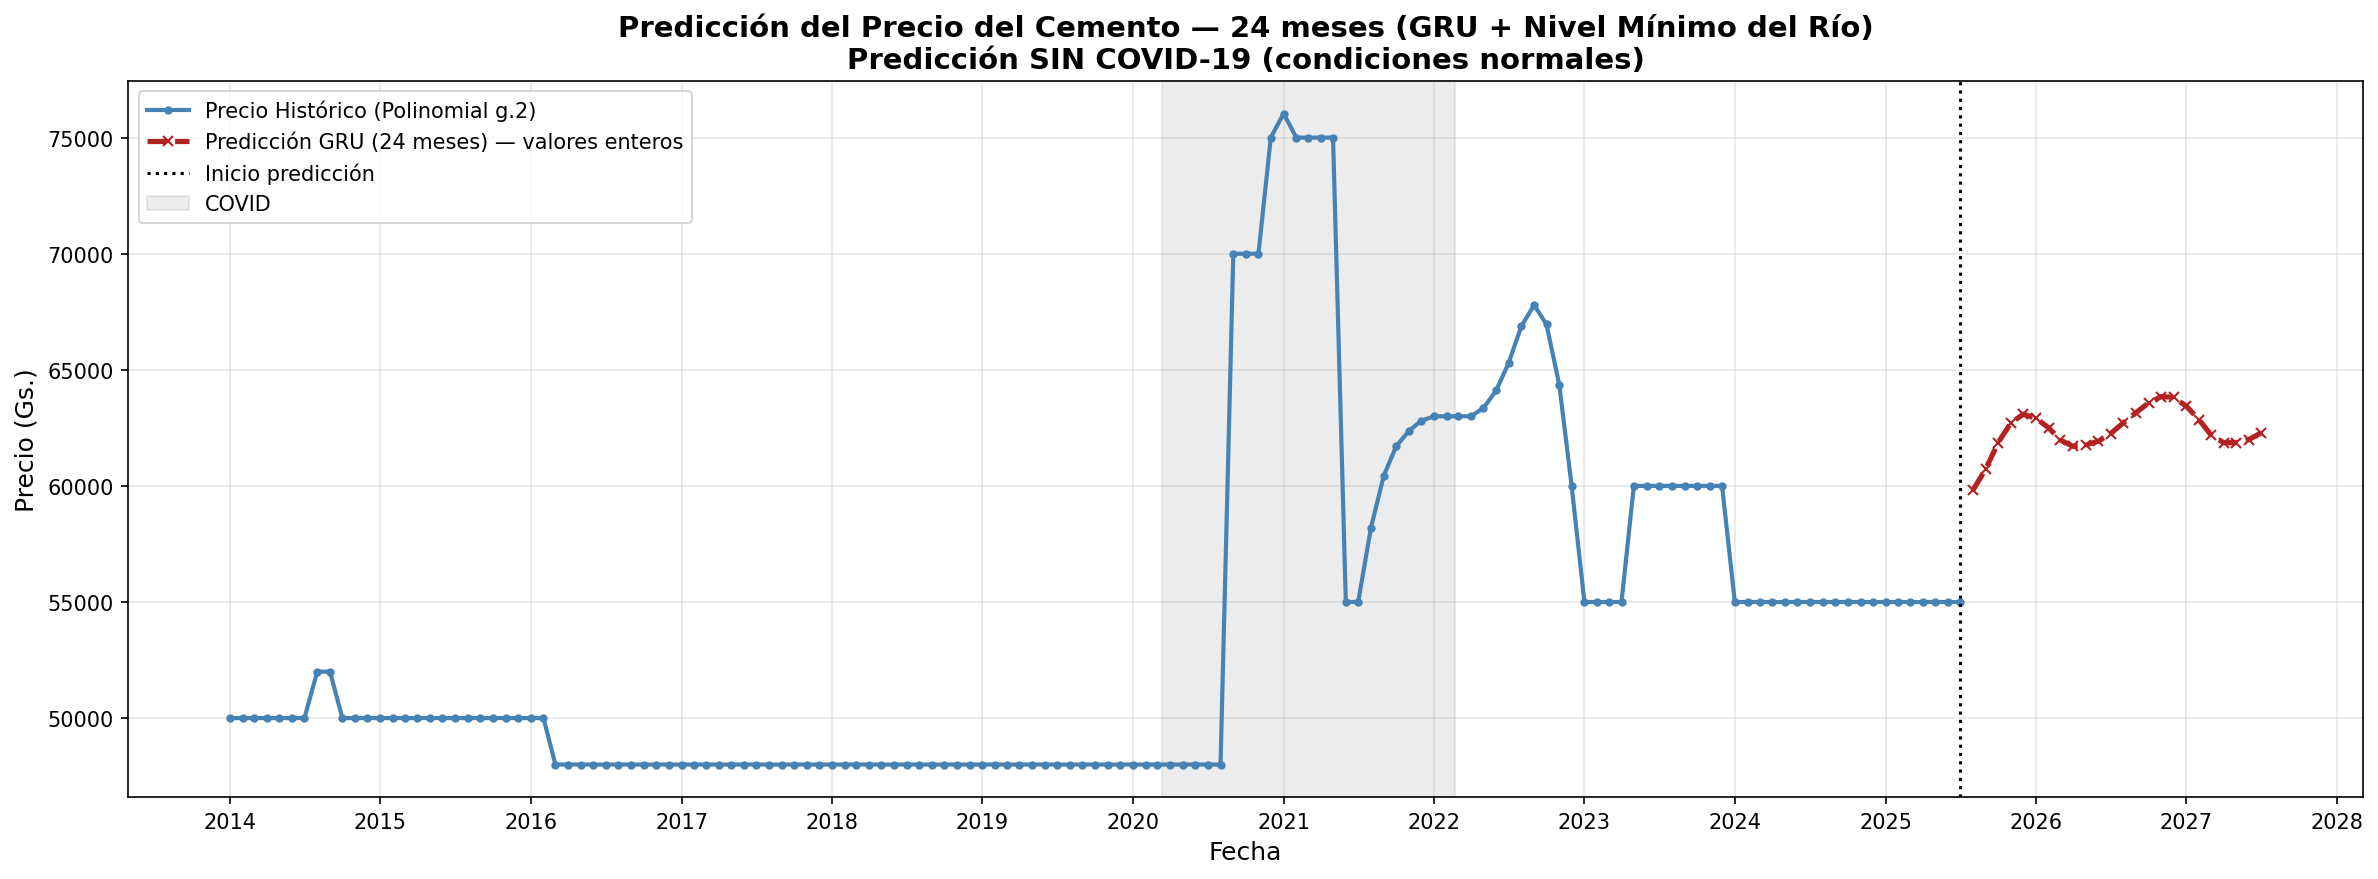
\includegraphics[width=0.75\textwidth]{../predicciones/prediccion_cemento_gru/prediccion_sin_covid/final_06_prediccion_futura_completa.png}

\vspace{0.1cm}
\begin{columns}
\begin{column}{0.5\textwidth}
\begin{itemize}\small
  \item RMSE Test: 4.964,27 Gs.
  \item Par\'ametros: 13.889
  \item Unidireccional
\end{itemize}
\end{column}
\begin{column}{0.5\textwidth}
\begin{itemize}\small
  \item AdamW (lr=0,0069)
  \item Lookback: 4 meses
  \item Pron\'ostico: 59.825--63.850 Gs.
\end{itemize}
\end{column}
\end{columns}
\end{frame}

% ============================================================
\begin{frame}{GRU Cemento --- Con Confinamiento}
\centering
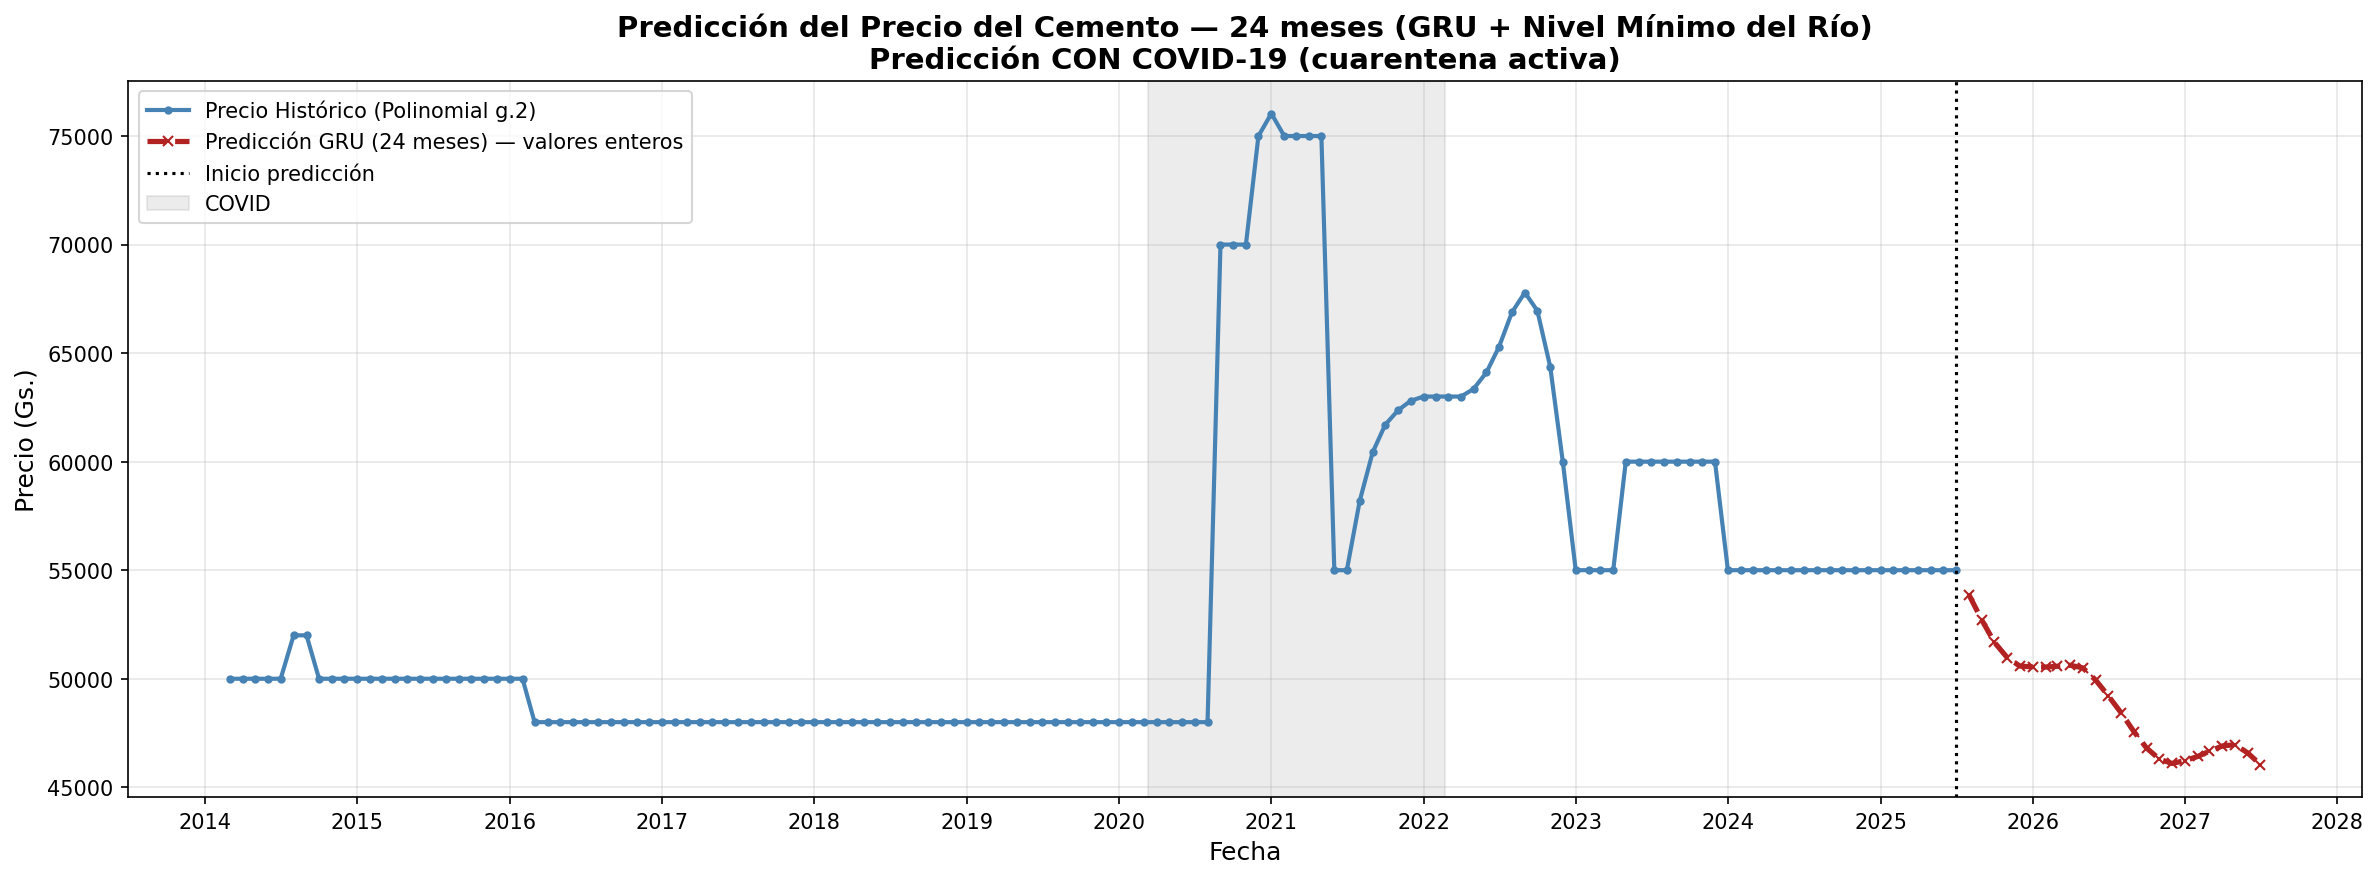
\includegraphics[width=0.75\textwidth]{../predicciones/prediccion_cemento_gru/resultados_con_covid/final_06_prediccion_futura_completa.png}

\vspace{0.1cm}
\begin{columns}
\begin{column}{0.5\textwidth}
\begin{itemize}\small
  \item RMSE Test: 4.964,27 Gs.
  \item Misma arquitectura GRU
  \item 13.889 par\'ametros
\end{itemize}
\end{column}
\begin{column}{0.5\textwidth}
\begin{itemize}\small
  \item Pron\'ostico: 59.825--65.334 Gs.
  \item \textbf{+2,3\,\%} incremento
  \item Residuos: ruido blanco ($p>0{,}05$)
\end{itemize}
\end{column}
\end{columns}
\end{frame}

% ============================================================
\begin{frame}{GRU Ladrillo --- Sin Confinamiento}
\centering
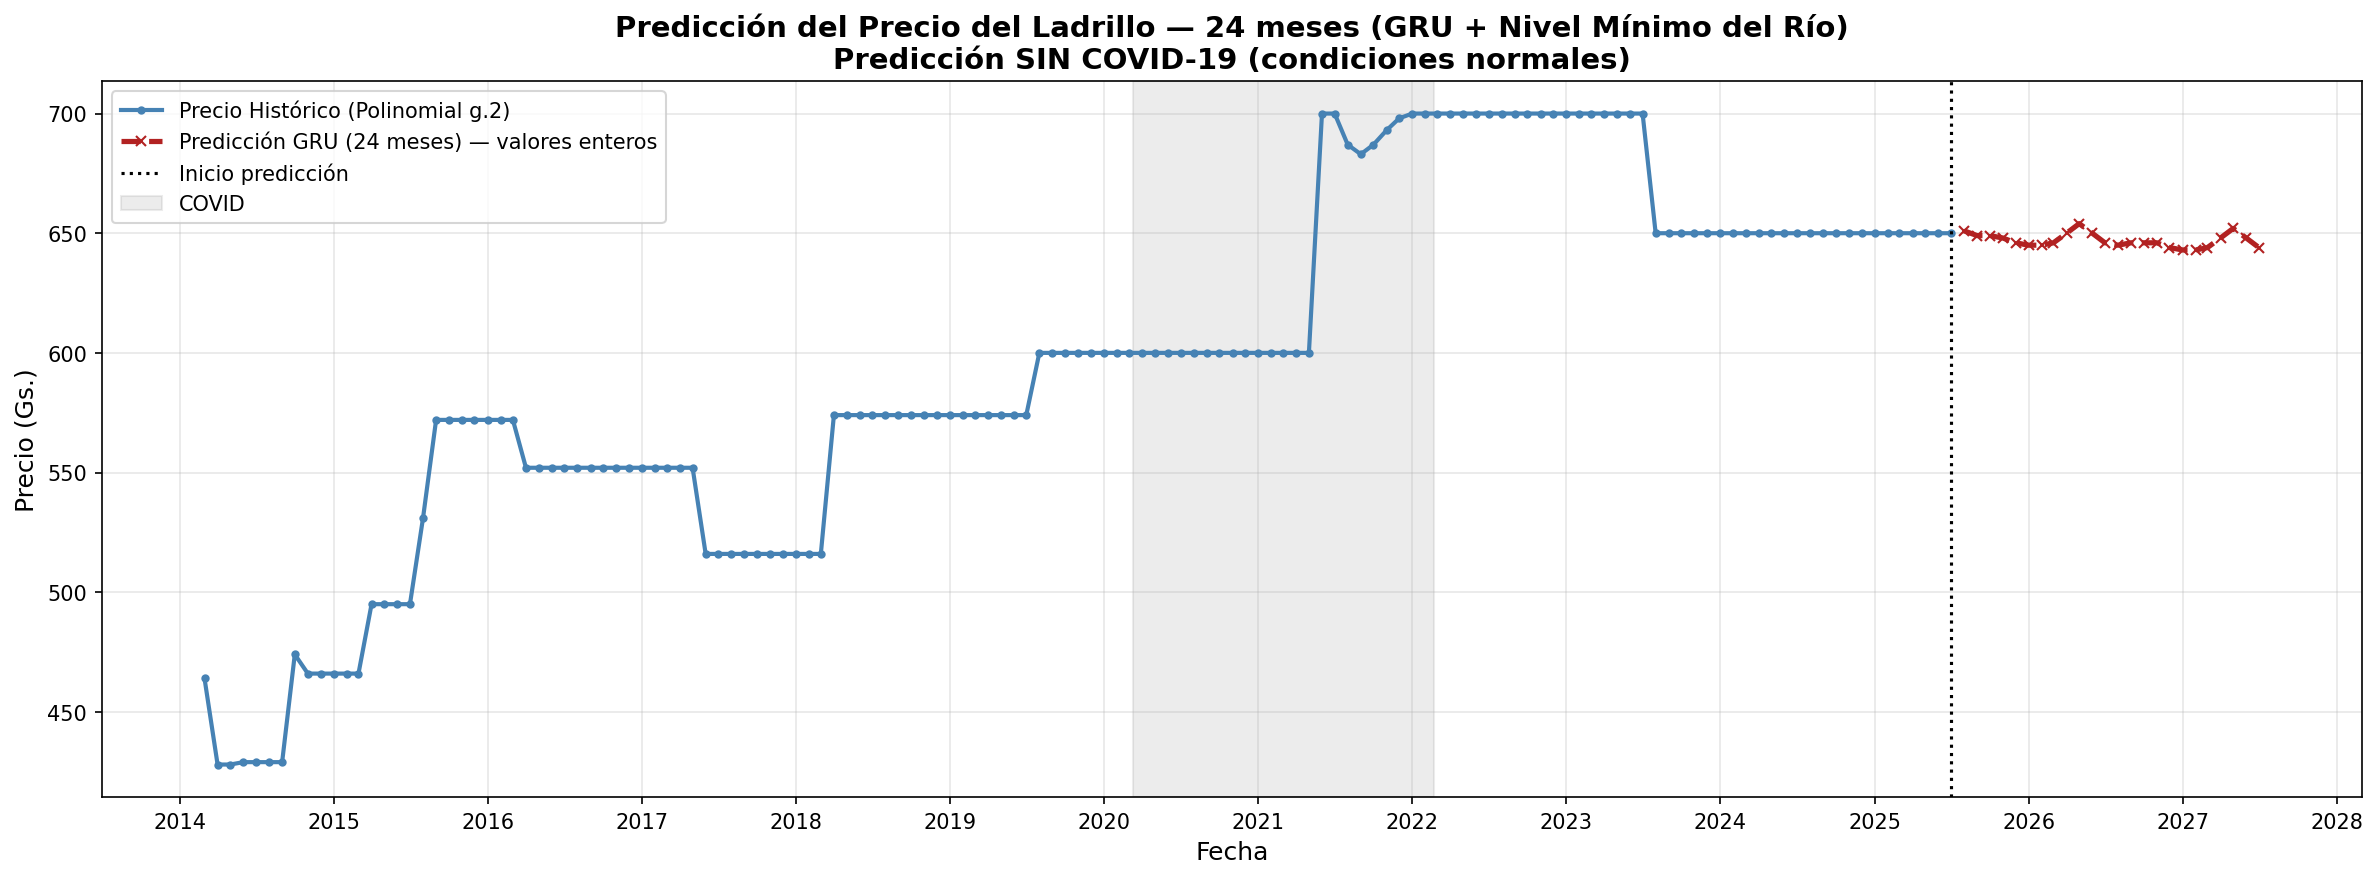
\includegraphics[width=0.75\textwidth]{../predicciones/prediccion_ladrillo_gru/resultados_sin_covid/final_06_prediccion_futura_completa.png}

\vspace{0.1cm}
\begin{columns}
\begin{column}{0.5\textwidth}
\begin{itemize}\small
  \item RMSE Test: 11,88 Gs.
  \item Par\'ametros: 13.889
  \item Unidireccional
\end{itemize}
\end{column}
\begin{column}{0.5\textwidth}
\begin{itemize}\small
  \item Adam (lr=0,0084)
  \item Lookback: 3 meses
  \item Pron\'ostico: 661--726 Gs.
\end{itemize}
\end{column}
\end{columns}
\end{frame}

% ============================================================
\begin{frame}{GRU Ladrillo --- Con Confinamiento}
\centering
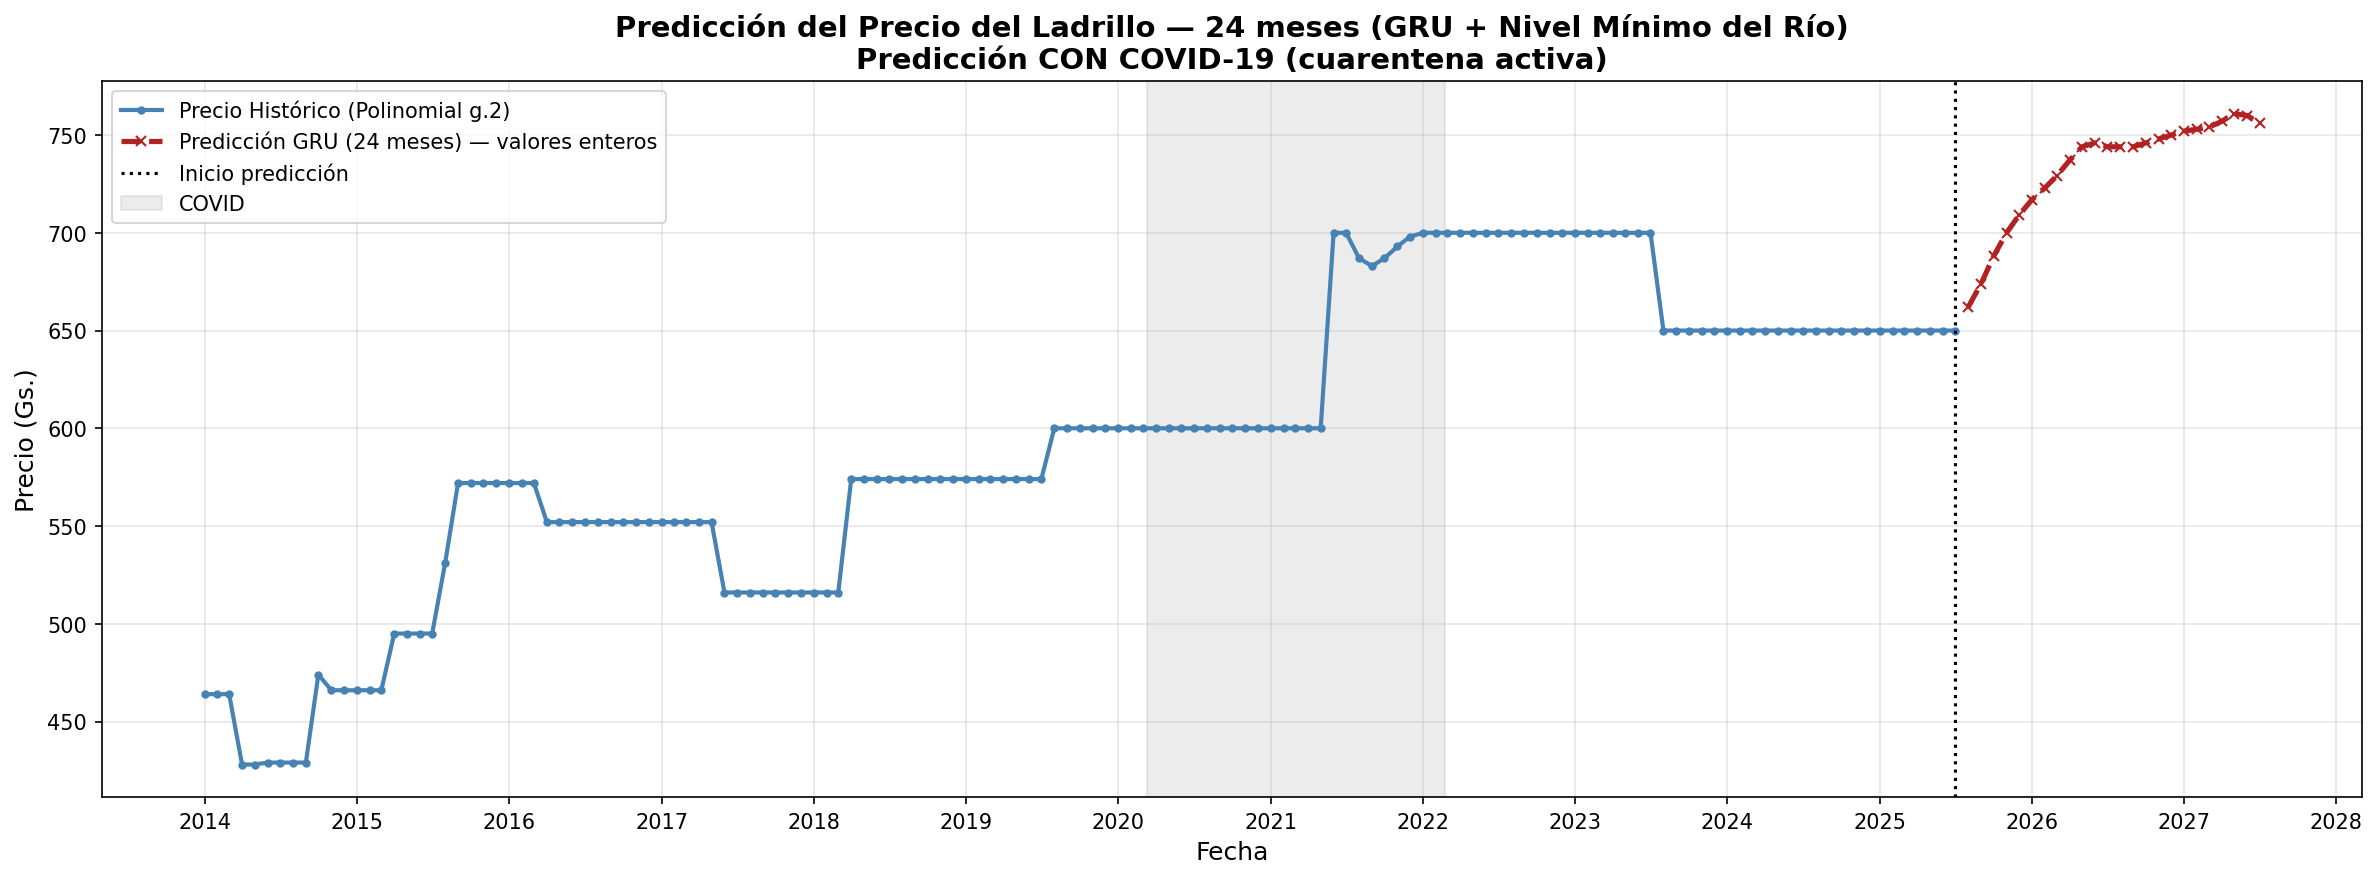
\includegraphics[width=0.75\textwidth]{../predicciones/prediccion_ladrillo_gru/resultados_con_covid/final_06_prediccion_futura_completa.png}

\vspace{0.1cm}
\begin{columns}
\begin{column}{0.5\textwidth}
\begin{itemize}\small
  \item RMSE Test: 11,11 Gs.
  \item Par\'ametros: 13.889
  \item Unidireccional
\end{itemize}
\end{column}
\begin{column}{0.5\textwidth}
\begin{itemize}\small
  \item Adam (lr=0,0098)
  \item Pron\'ostico: 659--763 Gs.
  \item \textbf{+5,1\,\%} incremento
\end{itemize}
\end{column}
\end{columns}
\end{frame}

% ============================================================
\section{Comparaci\'on y Discusi\'on}
% ============================================================

\begin{frame}{Comparaci\'on de Modelos}
\begin{table}[ht]
\centering
\small
\begin{tabular}{llrrl}
\toprule
\textbf{Modelo} & \textbf{Material} & \textbf{RMSE Test} & \textbf{Par\'ams} & \textbf{Observaci\'on} \\
\midrule
SARIMAX & Cemento  & 4.840 Gs.  & 3      & Paseo aleatorio \\
\rowcolor{verdeclaro} LSTM    & Cemento  & \textbf{4.395 Gs.}  & 36.481 & Mejor RMSE (bidirec.) \\
GRU     & Cemento  & 4.964 Gs.  & 13.889 & Residuos ruido blanco \\
\midrule
SARIMAX & Ladrillo & 4,55 Gs.   & 3      & Paseo aleatorio \\
\rowcolor{verdeclaro} LSTM    & Ladrillo & \textbf{6,62 Gs.}   & 36.481 & Bidireccional \\
GRU     & Ladrillo & 11,11 Gs.  & 13.889 & Unidireccional \\
\midrule
LSTM    & R\'io    & 0,046 m    & 1.075.713 & Univariado; 512 uds. \\
\bottomrule
\end{tabular}
\end{table}

\begin{itemize}\small
  \item \textbf{LSTM}: mejor RMSE en ambos materiales.
  \item \textbf{GRU}: residuos sin autocorrelaci\'on, arquitectura m\'as compacta.
  \item \textbf{SARIMAX}: sin estructura predictiva real.
\end{itemize}
\end{frame}

% ============================================================
\begin{frame}{Impacto del Confinamiento por COVID-19}
\begin{table}[ht]
\centering
\small
\begin{tabular}{llcc}
\toprule
\textbf{Modelo} & \textbf{Material} & \textbf{Efecto} & \textbf{Significativo?} \\
\midrule
SARIMAX & Cemento  & $-23{,}67$ Gs./mes & No ($p=1{,}000$) \\
SARIMAX & Ladrillo & $-0{,}83$ Gs./mes  & No ($p=0{,}999$) \\
\midrule
LSTM    & Cemento  & +16,5\,\% l\'im. sup. & S\'i \\
LSTM    & Ladrillo & +10,5\,\% l\'im. sup. & S\'i \\
\midrule
GRU     & Cemento  & +2,3\,\%             & S\'i \\
GRU     & Ladrillo & +5,1\,\%             & S\'i \\
\bottomrule
\end{tabular}
\end{table}

\vspace{0.2cm}
\begin{itemize}
  \item LSTM y GRU coinciden: \textbf{presi\'on ascendente} sobre los precios.
  \item El SARIMAX lineal no detecta efectos no lineales.
  \item La representaci\'on binaria es una simplificaci\'on del \textit{shock} real.
\end{itemize}
\end{frame}

% ============================================================
\begin{frame}{Discusi\'on}
\begin{itemize}
  \item \textbf{SARIMAX como paseo aleatorio:} sin t\'erminos AR/MA; competitivo en periodos estables, pero sin capacidad predictiva real.

  \vspace{0.2cm}
  \item \textbf{LSTM --- mejor RMSE pero residuos autocorrelados:}\\
  Cemento: autocorrelaci\'on significativa ($p=5{,}69 \times 10^{-5}$).

  \vspace{0.2cm}
  \item \textbf{GRU --- residuos como ruido blanco:}\\
  Mayor fiabilidad en intervalos de confianza. Desempe\~no comparable con 62\,\% menos par\'ametros.

  \vspace{0.2cm}
  \item \textbf{No existe un modelo universalmente superior:}\\
  La elecci\'on depende de las caracter\'isticas de la serie a predecir.
\end{itemize}
\end{frame}

% ============================================================
\section{Conclusiones}
% ============================================================

\begin{frame}{Conclusiones}
\begin{itemize}
  \item Es \textbf{viable} desarrollar investigaci\'on predictiva con recursos gratuitos (datos p\'ublicos + software libre).

  \vspace{0.15cm}
  \item Las RNNs (LSTM, GRU) son superiores al SARIMAX para capturar \textbf{patrones no lineales}.

  \vspace{0.15cm}
  \item Los modelos funcionan como herramientas de \textbf{inteligencia de negocios} para mitigar riesgo y optimizar planificaci\'on financiera.

  \vspace{0.15cm}
  \item \textbf{No existe un modelo universalmente superior}: LSTM mejor RMSE, GRU mejor calidad de residuos.

  \vspace{0.15cm}
  \item La variable de confinamiento act\'ua como se\~nal de \textbf{presi\'on ascendente} en ambas arquitecturas.
\end{itemize}
\end{frame}

% ============================================================
\begin{frame}{Trabajos Futuros}
\begin{enumerate}
  \item \textbf{Ampliar variables ex\'ogenas:}\\
  Precio del combustible, cotizaci\'on del d\'olar y otros indicadores.

  \vspace{0.4cm}
  \item \textbf{Extensi\'on a otros materiales:}\\
  Varillas, cal hidratada, otros tipos de ladrillos.

  \vspace{0.4cm}
  \item \textbf{Explorar modelos alternativos:}\\
  Transformers, modelos h\'ibridos (SARIMAX + LSTM), ensambles.
\end{enumerate}
\end{frame}

% ============================================================
\section{Referencias}
% ============================================================

\begin{frame}{Referencias}
\small
\begin{itemize}
  \item Mandu'a. (n.d.). Ediciones. \texttt{https://www.mandua.com.py/ediciones}
  \item Dir.\ de Meteorolog\'ia e Hidrolog\'ia. (n.d.). Nivel del R\'io.
  \item La Naci\'on. (2021). INC sufre sobrecosto por bajante del r\'io.
  \item Min.\ de Salud P\'ublica. (2020). Decretos COVID-19.
  \item Casta\~neda \& Aguirre (2022). Variabilidad de precios --- Valle del Cauca.
  \item Almada de Bernal et al.\ (2022). Variaci\'on de precios --- Ciudad del Este.
  \item Sosa-Cabrera et al.\ (2024). Feature selection: inter-attribute cooperation.
  \item Siami-Namini \& Namin (2018). ARIMA vs.\ LSTM.
  \item Kratzert et al.\ (2018). Rainfall-runoff modelling using LSTM.
  \item Cho et al.\ (2014). Learning phrase representations using RNN encoder-decoder.
\end{itemize}
\end{frame}

% ============================================================
% CIERRE
% ============================================================

\begin{frame}
\centering
\vspace{1cm}
{\Huge ?`Preguntas?}

\vspace{0.8cm}
{\Large Muchas gracias por su atenci\'on}

\vspace{0.8cm}
{\small Mat\'ias Rub\'en S\'anchez S\'anchez \quad -- \quad Diego Milciades Esp\'inola Alvarenga\\[0.2cm]
Tutor: Gustavo Sosa-Cabrera}

\vspace{0.5cm}

\includegraphics[height=1.2cm]{../images/logo_universidad_nacional.png}%
\hspace{1.5cm}%

\includegraphics[height=1.2cm]{../images/logo_fpuna.png}
\end{frame}

\end{document}
